\documentclass{book}
\usepackage[pdfauthor={}, pdftitle={}, pdfproduce={}, pdfcreator={}]{hyperref}
\usepackage{graphicx} % Required for inserting images
\usepackage{amsfonts}
\usepackage{amsmath}
\usepackage{amssymb}
\usepackage{amsthm}
\usepackage{pxfonts}
\usepackage[italian]{babel}
\title{Appunti di campi elettromagnetici e circuiti}
\author{Marco C}
\date{A.A. 24/25}

\begin{document}
\maketitle

\chapter*{Simbologia e grandezze fisiche}
    \section*{Simbologia}
    \begin{itemize}
        \item $\underline{v}$  vettore
        \item $\underline{\underline{A}}$ matrice
        \item $(\underline{a} \ | \ \underline{b})$ prodotto scalare fra due vettori
    \end{itemize}
    \section*{Grandezze fisiche}
    \begin{itemize}
        \item $\underline{e}$  campo elettrico $(\displaystyle \frac{N}{C})$
        \item $\underline{h}$  campo magnetico $(\displaystyle \frac{A}{m})$
        \item $\underline{b}$  campo d'induzione magnetica $(\displaystyle T)$
        \item $\underline{d}$  campo d'induzione elettrica (o spostamento elettrico) $(\displaystyle \frac{C}{m^{2}})$ 
    \end{itemize}
\chapter*{Disclaimer}
    Questo file di appunti \textbf{non} pretende di essere una sostituzione al corso tenuto dal Professor Capozzoli 
    né si spaccia per materiale prodotto dal professore stesso. Nel caso qualcuno si accorga di errori da segnalare può 
    farlo tramite una pull-request al repo github. \\ \\ \\ \\
    -Marco
\tableofcontents

\chapter{Fondamenti di Elettromagnetismo}
    \section{Le leggi di Maxwell}
        \subsection{Equazioni di Maxwell in forma differenziale}
        Partiamo dall'assunto che le equazioni di Maxwell siano corrette. Il fenomeno elettromagnetico è \textbf{unico} e non c'è campo elettrico senza quello magnetico. Questo si può vedere intuitivamente se si prova a correrre accanto ad un filo carico: un osservatore in movimento vedrà la generazione di un campo magnetico, in quanto il filo si muove nel suo sistema di riferimento, mentre uno fermo in un sistema solidale con il filo vedrà semplicemente un campo elettrico. \\
        \begin{align}
            \nabla \times \underline{e} = - \displaystyle \frac{\partial }{ \partial t}     \underline{b} \label{eqn:maxwell_rot_e} \\
            \nabla \times \underline{h} = \displaystyle \frac{\partial}{ \partial t} \underline{d}+\underline{j}  \label{eqn:maxwell_rot_h} \\
            \nabla \cdot \underline{d} = \rho  \label{eqn:maxwell_div_d}\\
            \nabla \times \underline{b} = 0 \label{eqn:maxwell_div_b}
        \end{align}
        Il fenomeno elettromagnetico è descritto da \textit{campi}. Un campo è una corrispondenza, cioè un oggetto che descrive la variazione di una grandezza fisica in funzione della sua posizione nello spazio e nel tempo. \\
        Dato un sistema di riferimento $Oxyz$, sia $\underline{r} = x \underline{i}_{x} + y \underline{i}_{y} + z \underline{i}_{z}$ un punto dello spazio tridimensionale.\\
        I campi che descrivono il fenomeno elettromagnetico sono quattro: il campo elettrico $\underline{e}$, il campo  magnetico $\underline{h}$ e quelli di induzione elettrica e magnetica $\underline{d}$ e $\underline{b}$. \\
        Tutti e quattro sono campi \textit{vettoriali}, ergo ritornano come risultato un vettore, nel nostro caso prendendo in ingresso il vettore $(\underline{r}, t)$.\\
        I campi che invece descrivono le cariche nello spazio e nel tempo sono il campo densità di corrente $\underline{j}$ ed il campo densità di carica $\underline{\rho}$. Il primo descrive in che modo si muovono le cariche nel tempo, costituendo dunque un campo vettoriale, mentre il secondo ci dice il valore della densità di carica, punto per punto ad ogni istante di tempo, ed è un campo \textit{scalare}, perché ritorna un numero (reale).\\
        La $\underline{j}$ e la $\underline{\rho}$ possono essere scritte come somma di un contributo \textit{impresso}, noto all'istante iniziale, ed un contributo \textit{incognito} che viene indotto dal campo. Allora la (\ref{eqn:maxwell_rot_h}) e la (\ref{eqn:maxwell_div_d}) possono essere riscritte come:
        \begin{align}
            \nabla \times \underline{h} = \displaystyle \frac{\partial}{\partial t} \underline{d}+ \underline{j} + \underline{j}_{0} \\
            \nabla \cdot \underline{d} = \rho + \rho_{0}
        \end{align}
        dove $\underline{j}_{0}$ e $\rho_{0}$ sono i valori noti di $\underline{j}$ e $\rho$ all'istante iniziale.\\
        \subsection{Quante informazioni servono affinché si trovi una soluzione?}
        Le equazioni di Maxwell sono problemi alle derivate parziali e dunque bisogna specificare le condizioni iniziali, che sono un insieme di condizioni \textit{sintetiche} per descrivere la situazione all'istante iniziale.\\ \\
        Il problema però si articola anche nello spazio, oltre che nel tempo. Considerato un dominio $V$, c'è bisogno di tener conto delle sorgenti di campi sia interne che esterne, ma per tener conto delle seconde bisognerebbe considerare tutto lo spazio ! Fortunatamente, se l'interazione è locale\footnote{Per locale noi intendiamo qualunque interazione avviene per step spaziali adiacenti, che è il caso della fisica classica} basta conoscere quali sono le \textit{condizioni al contorno}, cioè le condizioni dei campi al bordi del dominio considerato che tengono conto dell'effetto dei campi esterni.\\
        Per chiarire questa cosa consideriamo un dominio $D$ in due dimensioni $xy$ (perché fare un disegno tetradimensionale è difficile in questa tempolinea) che si evolve attraverso il terzo asse, quello temporale $t$:
        \begin{figure}[h!]
            \centering
            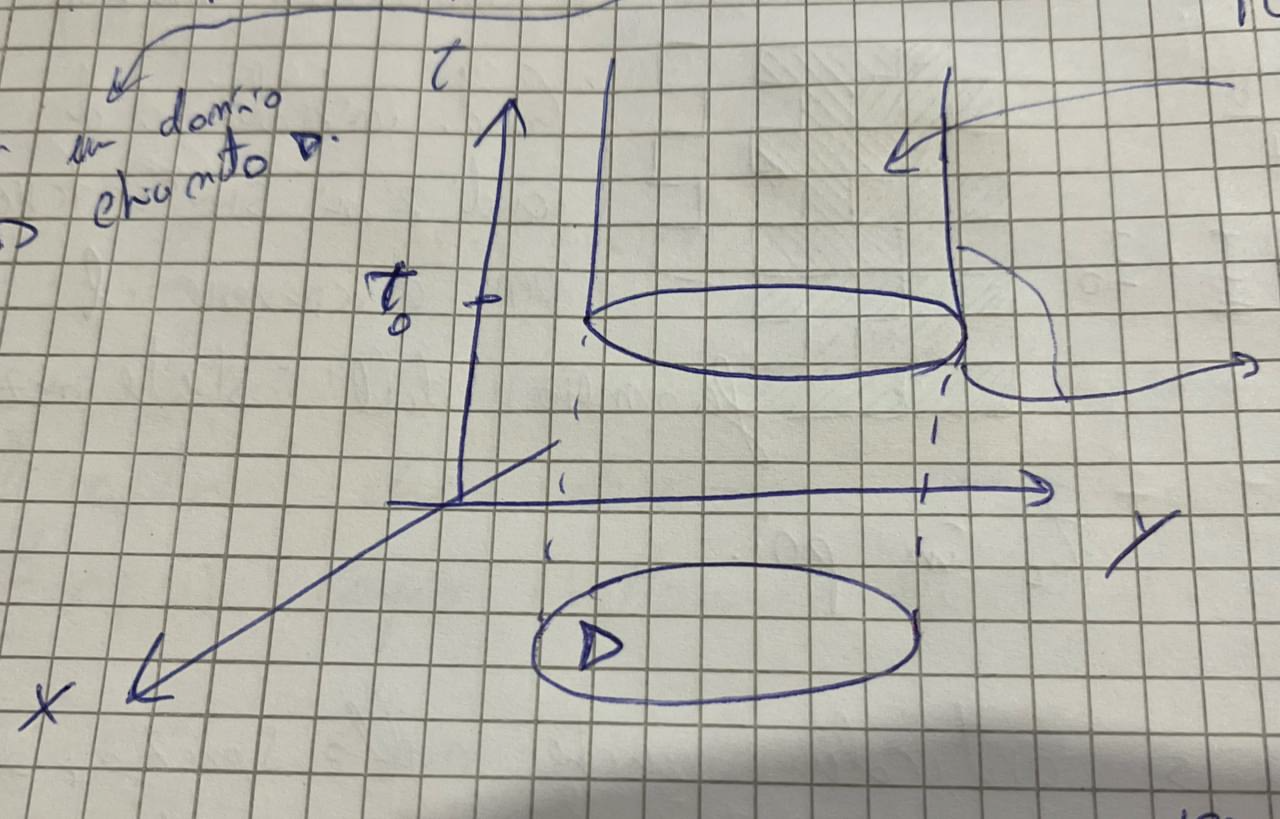
\includegraphics[width=0.5\linewidth]{img/Chapter_one/Chapt1img1.png}
            \caption{"Cilindro spaziotemporale"}
            \label{fig:chapt1img1}
        \end{figure} \\
        Fissato l'istante iniziale $t_{0}$ nel tempo si sviluppa un "cilindro spaziotemporale" all'interno del quale gli eventi (punti dello spazio tempo) relativi al fenomeno elettromagnetico di nostro interesse evolvono. Le sorgenti che influenzano i campi nella regione di spaziotempo interna al cilindro lo fanno passando per i bordi di tale dominio, e dunque vanno viste le condizioni iniziali e al contorno. \\ Le condizioni iniziali per $t_{0}$ devono trovarsi all'interno della base del cilindro e dunque l'unico constraint che hanno è che debbano accadere per $t_{0}$. Viceversa, le condizioni al contorno si trovano sulla superficie laterale del cilindro, libere di cambiare valore nel tempo ma ancorate alle stesse coordinate $(x,y)$ del contorno per ogni istante.\\ \\
        Ci sono 16 incognite per le equazioni di Maxwell, tre per ogni campo vettoriale ed una per $\rho$ che è un campo scalare, ma le equazioni sono otto, in quanto ce ne sono due vettoriali e due scalari. Dobbiamo allora specificare il mezzo all'interno del quale si propaga l'onda. Quese ulteriori relazioni si chiamano \textit{relazioni costitutive dei materiali}. \\ \\
        Quello che abbiamo scritto finora sono le equazioni di Maxwell in forma differenziale e sono equazioni \textit{locali}, cioè il valore dei campi viene calcolato punto per punto istante per istante. Le equazioni differenziali ci piaccino ma richiedono condizioni stringenti, ovvero la derivabilità dei campi ove ne si vuole conoscere il valore puntuale. Allora possiamo scrivere le equazioni in \textit{forma integrale}, che hanno più generalità e permettono di trattare le discontinuità senza problemi. 
        \subsection{Equazioni di Maxwell in forma integrale}
            Le equazioni di Maxwell in forma integrale hanno questa forma qua:
            \begin{align}
                \oint_{C} \underline{e} \cdot \underline{i_{l}} dl = - \frac{\partial}{\partial t}\iint_{S_{C}} \underline{b} \cdot \underline{i_{n}} dS \quad \\
                \oint_{C} \underline{h} \cdot \underline{i_{l}} dl = \frac{\partial}{\partial t} \iint_{S_{C}} \underline{d} \cdot \underline{i_{n}} dS + i(S_{c},t) \\
                \oiint_{\partial V} \underline{d} \cdot \underline{i_{n}} dS = q(V,t) \\
                \oiint_{\partial V} \underline{b} \cdot \underline{i_{n}}dS = 0
            \end{align}
        $C$ è una curva chiusa orientata, cioè esiste un vettore tangente $\underline{i_{l}}$ per cui non ci sono discontinuità nel suo evolvere lungo la curva. $S_{C}$ è la superficie che ha $C$ per bordo e versone normale $\underline{i_{n}}$ punto per punto, che deve essere anch'esso tale da essere continuo nel suo variare lungo la superficie, affinché questa sia orientabile.\\
        I due orientamenti di $C$ ed $S_{C}$ devono essere \textbf{coerenti}, cioè si opera secondo la regola della mano destra: si prende il verso del versore $\underline{i_{l}}$ con tutte le dita tranne il pollice, mentre con quest'ultimo si prende di conseguenza il verso del versore $\underline{i_{n}}$. \\ \\
        La corrente $i(S_{C}, t)$ è per definizione la quantità di carica netta per istante di tempo che passa attraverso la superficie $S_{C}$ in verso concorde alla normale $\underline{i_{n}}$ di tale superficie. Cariche positive con verso concorde alla normale danno contributo positivo, mentre cariche negative con verso concordo alla normale danno contributo negativo e viceversa per versi discordi alla normale. \\ \\
        Nella III e la IV equazione di Maxwell appaiono i flussi di campo di induzione elettrica e magnetica, che per convenzione sono scelti \textbf{uscenti}. Il valore $q(V,t)$ è la quantità di carica all'interno del volume $V$ nell'istante di tempo $t$. \\ \\ 
        Queste equazioni (integrali ndr) non sono locali perché fissato l'istante di tempo bisogna conoscere il valore dei campi su tutte le superfici o curve considerate. Per esempio, per conoscere la quantità di carica $q(V,t)$ all'interno della superficie $V$, bisogna conoscere il valore di $\underline{d}(\underline{r},t)$ su tutta la superficie $\partial V$. \\
        Inoltre, la corrispondenza $(V,t) \to q(V,t)$ non è una funzione numerica, perché $V$ è un volume, cioè un insieme di punti nel piano tridimensionale. Dunque si sta associando un insieme ed un tempo ad un valore $q(V,t)$ relativo ad un insieme ed un tempo. A noi interessa un'espressione numerica e dunque si può pensare di dividere $q(V,t)$ per il volume $V$ in esame e fare il limite, ottenendo la \textbf{densità volumica di carica}:
        \begin{equation}
            \rho(\underline{r},t) = \lim_{V \to 0} \frac{q(V,t)}{\textrm{meas}(V)}
        \end{equation}
        dove $\textrm{meas}(V)$ è la \textit{misura} di $V$, ovvero il valore del volume. La densità volumica è un campo scalare e si misura in $C/m^{3}$. Se ora consideriamo due volumi $V_{1}$ e $V_{2}$, che suppponiamo disgiunti, allora si può affermare:
        \begin{equation}
            q(V_{1} \cup V_{2}, t) = q_{1}(V_{1},t) + q_{2}(V_{2},t) \quad \quad \textrm{se} V_{1} \cap V_{2} = \emptyset
        \end{equation}
        Si può dimostrare che si può passre dalla densità di carica alla carica contenuta in un volume $V$ semplicemente integrando la densità di carica in tutto $V$:
        \begin{equation}
           \label{eqn:integrale_densitaCarica}
            q(V,t) = \iiint_{V} \rho(\underline{r},t)
        \end{equation}
        Il risultato di (\ref{eqn:integrale_densitaCarica}) è intuibile se si considerano tanti piccoli pezzettini disguinti $\Delta V$ così piccoli per i quali il rapporto fra la quantità di carica $dq$ dentro ogni volumetto $\Delta V$ ed il volumetto stesso è praticamente $\rho(\underline{r}, t)$. Dunque sommando tutti questi piccoli contributi e arrivando al limite si ottiene di nuovo la carica totale:
        \begin{equation}
            \frac{dq(\underline{r},t)}{\Delta V} \simeq \rho(\vec{r},t) \implies q \simeq \sum_{i}\Delta V_{i}\rho_{i}(\underline{r},t)
        \end{equation}
        Per la III equazione di Maxwell dividendo ambo membri per la misura di $V$ e facendo il limite:
        \begin{equation}
            \lim_{V \to 0} \frac{1}{\textrm{meas}(V)} \oiint_{\partial V} \underline{d} \cdot \underline{i_{n}} dS = \lim_{V \to 0} \frac{q(V,t)}{\textrm{meas}(V)}
        \end{equation}
        A secondo membro abbiamo la densità di carica mentre al primo abbiamo la definizione della divergeza di $\underline{d}$:
        \begin{equation}
        \label{eqn:def_divergenza}
            \textrm{div}(\underline{d}) = \lim_{V \to 0} \frac{1}{\textrm{meas}(V)} \oiint_{\partial V} \underline{d} \cdot \underline{i_{n}} dS 
        \end{equation}
        che noi scriviamo come prodotto scalare fra l'operatore $\nabla$ e $\underline{d}$. Ricordiamo che $\nabla$ scritto come vettore:
        \begin{equation}
            \nabla = (\frac{\partial }{\partial x}, \frac{\partial }{\partial y}, \frac{\partial }{\partial z})
        \end{equation}
        è puramente rappresentativo perché è un operatore. Con questo arteficio possiamo infatti scrivere:
        \begin{equation}
            \textrm{div}(\underline{d}) = \sum_{i} \frac{\partial}{\partial x_{i}}d_{i}
        \end{equation}
        fermo restando che la definizione della divergenza rimane la (\ref{eqn:def_divergenza}). La divergenza è uno strumento importante che ci permette di studiare la \textit{densità di flusso} in modo puntuale. Lo stesso ragionamento si può effettuare per la IV equazione di Maxwell per ottenere la forma locale.\\ \\
        Consideriamo ora una superficie $\Sigma$. La corrente che passa attraverso $\Sigma$ è definita come:
        \begin{equation}
            \lim_{\Delta t \to 0} \frac{q(\underline{\Sigma}, t + \Delta t)}{\Delta t} = i(\underline{\Sigma}, t)
        \end{equation}
        La corrente così definita non è un concetto puntuale perché perché la dipendenza da $\underline{\Sigma}$ presuppone quella dal \textit{versore} normale a $\Sigma$. \\
        Per capire meglio questa cosa ed in che modo è un problema, definiamo la densità di corrente:
        \begin{equation}
            \underline{j}(\underline{r}, t) = \lim_{\Sigma \to 0} \frac{i(\underline{\Sigma},t)}{\textrm{meas}(\Sigma)}
        \end{equation}
        Questa definizione non è completa, perché bisogna tener conto della dipendenza dall'orientamento della normale nel punto nel quale è collassata la superficie $\Sigma$, ergo bisogna più correttamente scrivere:
        \begin{equation}
            \underline{j}_{n}(\underline{r},t)
        \end{equation}
        Si ottiene l'espressione di un campo solo quando si specifica la normale $\underline{i}_{n}$, ottenendo dunque per ogni punto infiniti possibili campi (per ogni singola normale che si può prendere a partire da un punto). Questa è male perché a noi interessa l'espressione di un campo, cioè un oggetto per il quale date le coordinate spaziotemporale (ovvero quattro numeri) si ottiene un'altra grandezza. \\
        Abbiamo scritto $\underline{j}_{n}$ con la notazione utilizzata per i campi vettoriali, dunque vediamo come ci si arriva. Consideriamo un tetraedro nel piano tridimensionale $Oxyz$.
        \begin{figure}[h!]
            \centering
            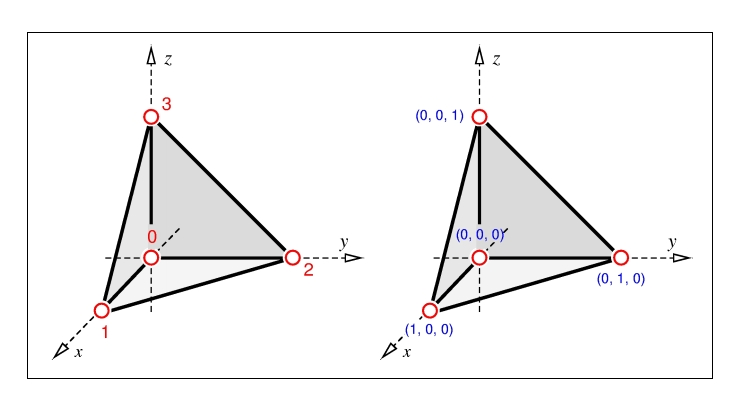
\includegraphics[width=0.75\linewidth]{img//Chapter_one/Chapt1img2.png}
            \caption{Immagine a puro scopo illustrativo}
        \end{figure}
        Assumiamo per ora valido il principio di conservazione per la carica (vedremo più avanti in che modo questo viene incluso nelle equazioni di Maxwell). Considerato un volume $V$ contenente carica $q(V,t)$ all'istante di tempo $t$, vale:
        \begin{equation}
        \label{eqn:conservazione_carica}
            \frac{\partial}{\partial t}q(V,t) = - i(\partial \underline{V},t)
        \end{equation}
        Questa relazione è inutitiva se si pensa, per esempio, a della carica negativa uscente. Questo implica che la derivata è positiva (perché carica negativa uscente = carica positiva entrante) ma carica negativa concorde al verso della normale implica corrente negativa, relazione verificata dalla (\ref{eqn:conservazione_carica}). \\
        Se chiamiamo i versori delle tre facce giacenti sui piani $\Sigma_{x}, \Sigma_{y}, \Sigma_{z}$ e quello della faccia "obliqua" $\Sigma_{n}$, non è difficile vedere che $\Sigma_{x}$ è normale al piano $yz$ e così via per $\Sigma_{y}$ e $\Sigma_{z}$. Allora scegliendo i versori $\Sigma_{i}$ ($i \in [x,y,z]$) concordi a quelli degli assi, questi risultano entranti nel tetraedro. Scegliamo, per convenzione, $\Sigma_{n}$ uscente dalla faccia obliqua. In condizioni stazionarie le derivate si annullano, risultato matematico che corrisponde nel nostro caso a carica netta entrante nel tetraedro pari a zero. Alla luce di ciò possiamo scrivere:
        \begin{equation}
            0 = i(\partial \underline{V}, t) = i(\underline{\Sigma}_{n}, t)+i(\underline{-\Sigma}_{x},t)+i(\underline{-\Sigma}_{y},t)+i(\underline{-\Sigma}_{z},t) = 0
        \end{equation}
        da cui si ottiene, intuitivamente, che il flusso di corrente entrante per le tre facce giacenti sui piani generati dai tre assi è pari a quello uscente dalla quarta superficie:
        \begin{equation}
            i(\underline{\Sigma}_{n}, t) = \sum_{k} i(\underline{\Sigma}_{k}, t) \qquad \qquad k \in (x,y,z)
        \end{equation}
        Scriviamo allora l'espressione in questo modo:
        \begin{equation}
            \frac{i(\underline{\Sigma}, t)}{\textrm{meas}(\underline{\Sigma}_{n})} = \sum_{k} \frac{i(\underline{\Sigma_{k}},t)}{\textrm{meas}(\Sigma_{k})} \frac{\textrm{meas}(\Sigma_{k})}{\textrm{meas}(\Sigma_{n})}
        \end{equation}
        dove $k \in (x,y,z)$. Facendo collassare il volume al punto (che poi corrisponde all'origine del nostro sistema di riferimento) si ottiene:
        \begin{align}
            \frac{i(\underline{\Sigma_{n}})}{\textrm{meas}(\Sigma_{n})} \to j_{n}(\underline{r},t) \\
            \frac{i(\underline{\Sigma_{k}})}{\textrm{meas}(\Sigma_{k})} \to j_{k}(\underline{r},t) \qquad \forall k
        \end{align}
        Il problema ora è vedere come collassa il rapporto:
        \begin{equation}
            \frac{\textrm{meas}(\Sigma_{k})}{\textrm{meas}(\Sigma_{n})}
        \end{equation}
        Se consideriamo il collasso bidimensionale del tetraedro su una delle facce, per esempio $x$, lavoriamo con il triangolo:
        \begin{figure}[h!]
            \centering
            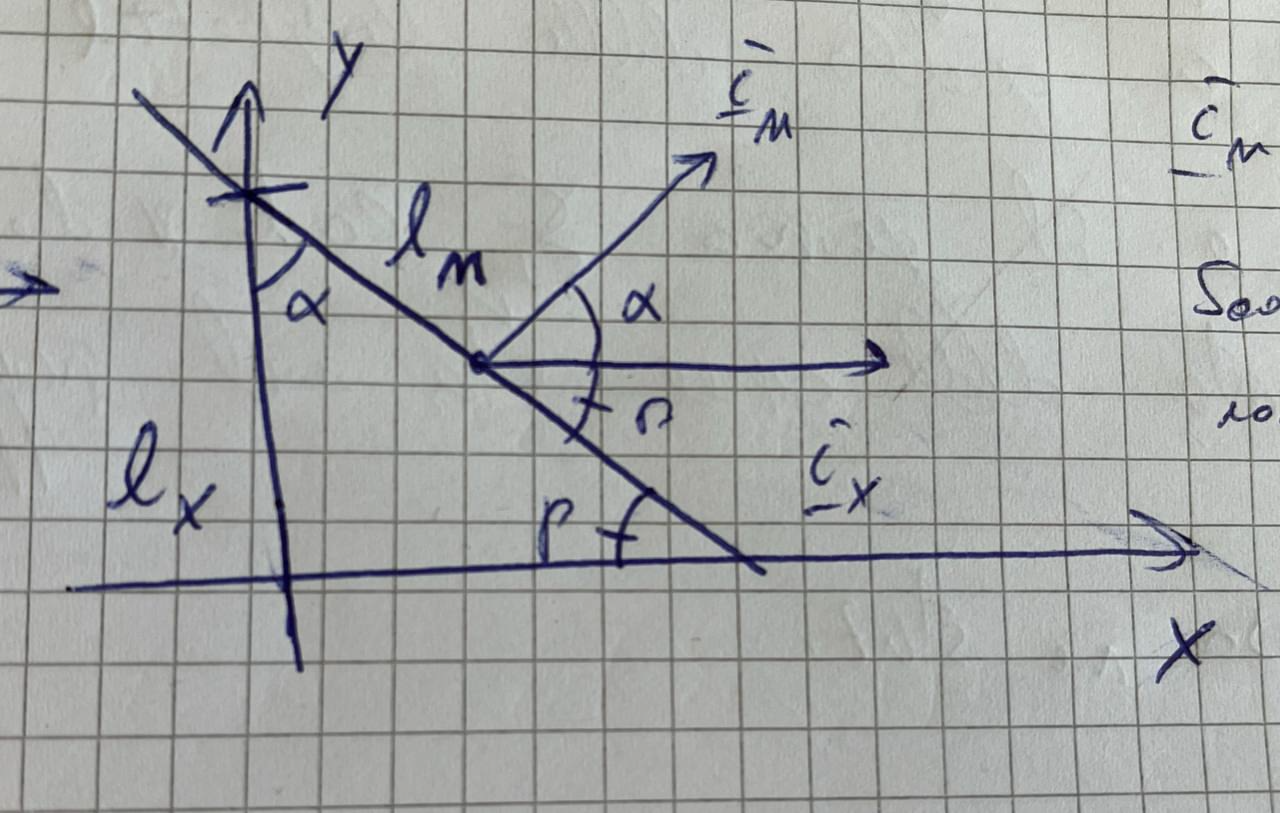
\includegraphics[width=0.75\linewidth]{img//Chapter_one/chap1img3.png}
            \caption{}
        \end{figure}
        La normale $\underline{i}_{n}$ alla superficie $\Sigma_{z}$ e quella $\underline{i}_{x}$ alla superficie $\Sigma_{x}$ formano un angolo $\alpha$ pari a quello formato dalle rette giacenti sulle due superfici. Dal momento che il rapporto fra le aree dei due triangoli (nel disegno 3D) corrispondenti alle facce $\Sigma_{x}$ e $\Sigma_{n}$ si riduce al rapporto fra le altezze (in quanto suddetti triangoli condividono la base), allora si può scrivere:
        \begin{equation}
            \frac{\textrm{mis}(\Sigma_{x})}{\textrm{mis}(\Sigma_{n})} = \frac{l_{x}}{l_{n}} = \cos{(\alpha)} = \underline{i}_{n} \cdot \underline{i}_{x}
        \end{equation}
        L'ultimo passaggio è giustificato dalla definizione di prodotto scalare fra due vettori e tenendo conto che i versori hanno modulo unitario.\\
        A valle di ciò che abbiamo detto possiamo scrivere la stessa cosa per le altre due dimensioni ed ottenere:
        \begin{equation}
            j_{n}(\underline{r},t) = j_{x}(\underline{r},t)(\underline{i}_{x}\cdot \underline{i}_{n})+j_{x}(\underline{r},t)(\underline{i}_{y}\cdot \underline{i}_{y})+j_{z}(\underline{r},t)(\underline{i}_{z}\cdot \underline{i}_{n})
        \end{equation}
        che riscriviamo come:
        \begin{equation}
            j_{n}(\underline{r},t) = (j_{x}\underline{i}_{x}+j_{y}\underline{i}_{y}+j_{z}\underline{i}_{z}) \cdot \underline{i}_{n} = \underline{j}(\underline{r},t) \cdot \underline{i}_{n}
        \end{equation}
        dove $\underline{j}(\underline{r},t)$ è il vettore densità di corrente. Dunque è possibile ottenere la densità di corrente relativa ad una superficie tramite il prodotto scalare fra il vettore densità di corrente ed il versore normale alla superficie stessa.\\
        Ovviamente è possibile tornare indietro:
        \begin{equation}
            i(\underline{\Sigma}, t) = \iint_{\Sigma} \underline{j} (\underline{r},t) \cdot \underline{i}_{n} d \Sigma
         \end{equation}
         Nel caso non stazionario valgono le stesse relazioni che abbiamo appena trovato. Dimostriamolo considerando l'espressione che tiene conto delle derivate non nulle:
         \begin{equation}
             i(\underline{\Sigma}_{n}, t) = \sum_{k} i(\underline{\Sigma}_{k},t) - \frac{\partial}{\partial t}q
         \end{equation}
         che sotto l'ipotesi di poter passare le derivate sotto il segno d'integrale scriviamo nella forma più comoda:
         \begin{equation}
             i(\underline{\Sigma}_{n}, t) = \sum_{k} i(\underline{\Sigma}_{k},t) - \iiint_{V} \frac{\partial}{\partial t}\rho
         \end{equation}
        Come in precedenza, possiamo dividere ambo membri per $\textrm{meas}(\Sigma_{n})$, ma dobbiamo capire dove converge il rapporto:
        \begin{equation}
            \frac{\displaystyle\iiint_{V} \frac{\partial}{\partial t}\rho}{\textrm{meas}(\Sigma_{n})}
        \end{equation}
        Per il teorema della media esiste un $\rho_{0}$ tale per cui:
        \begin{equation}
            \iint_{V} \frac{\partial}{\partial t} \rho dV = \frac{\partial \rho}{\partial t} |_{\rho = \rho_{0}} \cdot \textrm{meas}(V)
        \end{equation}
        Poiché $\textrm{meas}(V)$ va a zero più velocemente di $\textrm{meas}(\Sigma_{n})$, cioè è un infinitesimo di ordine superiore rispetto a $\textrm{meas}(\Sigma_{n})$, allora il contributo associato alla variazione della carica interna al volume è nullo, ragion per la quale quanto detto per il caso stazionario vale anche nel caso non stazionario. \\ \\
        Ora che abbiamo capito perché la corrente, che è una quantità scalare, ha come densità una quantità vettoriale, consideriamo la II° equazione di Maxwell\footnote{Qui andrebbe scritto a secondo membro il contributo della densità di corrente come $\iint_{S_{C}} \underline{j} \cdot \underline{i}_{n}dS$, ma la dipendenza della corrente dalla superficie considerata è contenuta nella dipendenza di questa dal proprio versore, che quindi viene esplicitato quando si scrive la corrente come flusso della densità di corrente}:
        \begin{equation}
            \oint_{C} \underline{h} \cdot \underline{i}_{l} dl = \frac{\partial}{\partial t} \iint_{S_{C}} \underline{d} \cdot \underline{i}_{n}dS + \frac{\partial}{\partial t} \iint_{S_{C}} i(\underline{S}_{C}, t)dS
        \end{equation}
        
        Per arrivare ad esplicitare la forma locale della II° legge, consideriamo tre casi elementari sui quali si possono costruire quelli più complessi, ovvero l'applicazione della legge su piani con normali corrispondenti ai tre assi di riferimento. Esaminiamo il caso di una superficie piana $S_{C_{x}}$ con contorno $C_{x}$ e normale $\underline{i}_{x}$. Gli altri due casi con $\underline{i}_{y}$ ed $\underline{i}_{z}$ si ricavano in modo analogo. 
        \begin{figure}[h!]
            \centering
            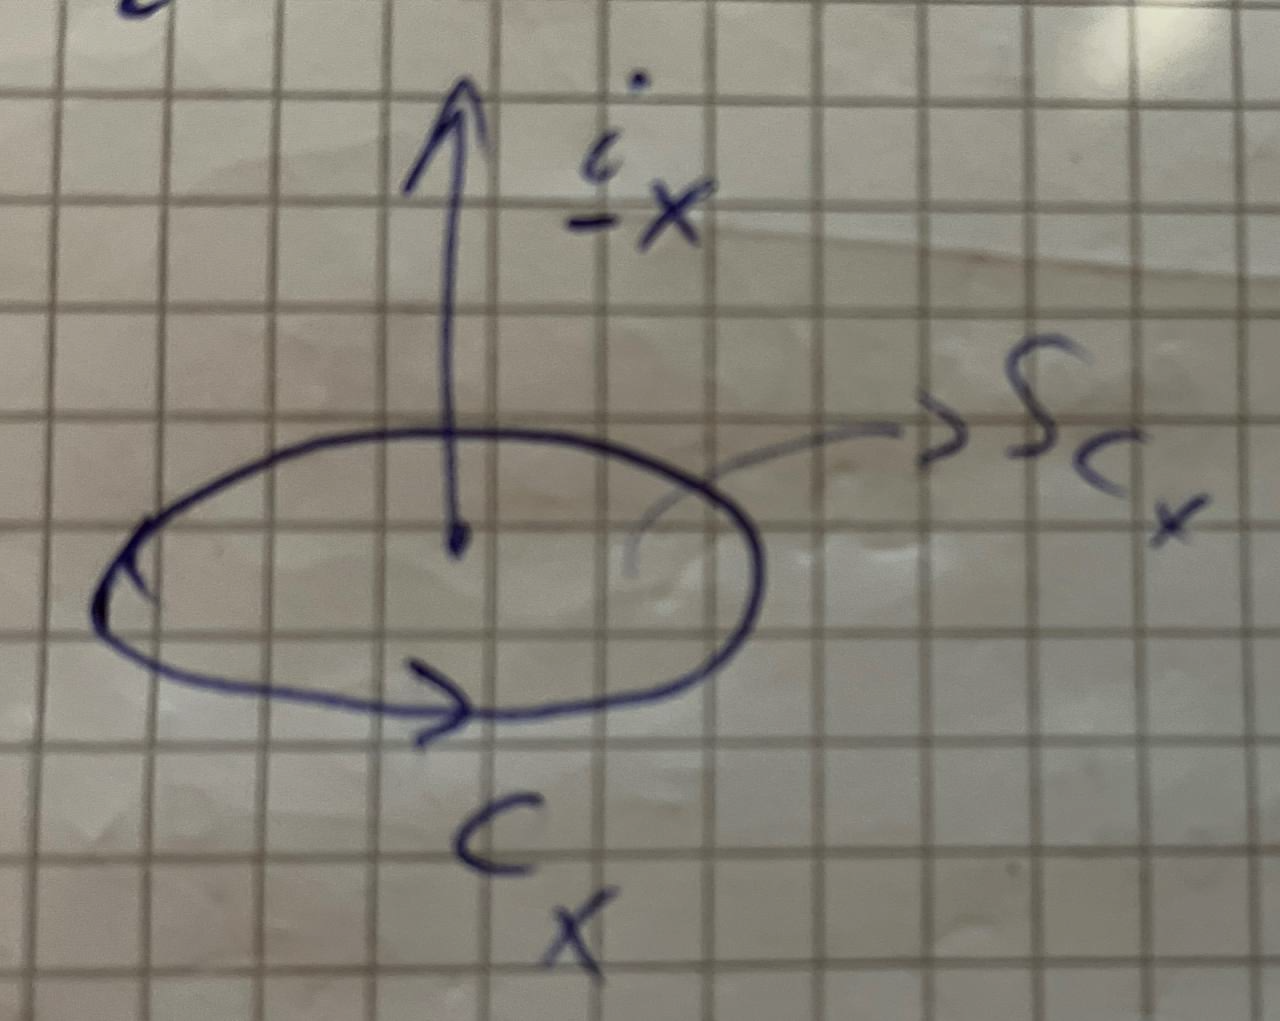
\includegraphics[width=0.35\linewidth]{img//Chapter_one/Chapt1img4age.png}
            \caption{}
        \end{figure}
        Dividiamo per $\textrm{meas}(S_{C_{x}})$
        \begin{equation}
            \frac{\displaystyle \oint_{C_{x}} \underline{h} \cdot \underline{i}_{l}dl}{\textrm{meas}(S_{C_{x}})} = \frac{\partial}{\partial t} \frac{\displaystyle \iint_{S_{C_{c}}} \underline{d} \cdot \underline{i}_{n}dS}{\textrm{meas}(S_{C_{x}})} + \frac{\partial}{\partial t} \frac{i(\underline{S_{c}}, t)}{\textrm{meas}(S_{C_{x}})}
        \end{equation}
        Facendo collassare la superficie ad un punto otteniamo la densità di corrente al secondo pezzo del membro di destra, mentre il primo termine di destra lo scriviamo come:
        \begin{equation}
            \frac{\partial}{\partial t} \frac{\displaystyle \iint_{S_{C_{x}}} \underline{d} \cdot \underline{i}_{n} dS}{\textrm{meas}(S_{C_{x}})} = \frac{\displaystyle  \iint_{S_{C_{x}}} \frac{\partial}{\partial t} \underline{d} \cdot \underline{i}_{n} dS}{\textrm{meas}(S_{C_{x}})}  
        \end{equation}
        sotto l'ipotesi che si possa passare la derivata sotto il segno di integrale. Nel nostro caso $\underline{i}_{n} = \underline{i}_{x}$ e dunque moltiplicare $\underline{d}$ per $\underline{i}_{x}$ equivale a prelevare la componente di $\underline{d}$ lungo $x$:
        \begin{equation}
            \frac{\displaystyle  \iint_{S_{C_{x}}} \frac{\partial}{\partial t} d_{x} \ dS}{\textrm{meas}(S_{C_{x}})}  
        \end{equation}
        Per il teorema della media questa quantità è pari a:
        \begin{equation}
            \frac{\partial}{\partial t}|_{x=x_{0}} \frac{\textrm{meas}(S_{C_{x}})}{\textrm{meas}(S_{C_{x}})} = \frac{\partial}{\partial t} d_{x}|_{x=x_{0}}
        \end{equation}
        dove $x_{0}$ è il punto nel quale la superficie collassa. \\
        Introduciamo a questo punto il \textbf{rotore} come \textit{densità di circuitazione} per esprimere la quantità del membro di sinistra. La componente lungo $x$ del rotore è definita come:
        \begin{equation}
            \textrm{rot}_{x}(\underline{h}) = \lim_{S_{C_{x}} \to x_{0}} \frac{\displaystyle \oint \underline{h} \cdot \underline{i}_{x} dl}{\textrm{meas}(S_{C_{x}})}
        \end{equation}
        Di nuovo, il gradiente si può esprimere in modo simbolico come abbiamo fatto con la divergenza come:
        \begin{equation}
            \textrm{rot}(\underline{h}) = \nabla \times \underline{h} = \begin{vmatrix} i_{x} & i_{y} & i_{z} \\ \frac{\partial}{\partial_{x}} & \frac{\partial}{\partial_{y}} & \frac{\partial}{\partial_{z}}  \\ h_{x} & h_{y} & h_{z} \end{vmatrix}
        \end{equation}
        Per le altre due componenti del rotore la definizione è analoga, basta fare il prodotto scalare con i versori $\underline{i}_{y}$ e $\underline{i}_{z}$. Si può tornare indietro integrando:
        \begin{equation}
            \oint_{C_{x}} \underline{h} \cdot \underline{i}_{x} dl = \iint_{S_{C_{x}}} \nabla \times \underline{h} \cdot \underline{i}_{x} dS
        \end{equation}
        che esteso alle tre dimensioni non è nient'altro che il teorema di Stokes\footnote{"The line integral of a vector field over a loop is equal to the surface integral of its curl over the enclosed surface."}
        \\
        In definitiva otteniamo:
        \begin{equation}
            \iint_{S_{C}} \nabla \times \underline{h} \cdot \underline{i}_{n} dS = \frac{\partial}{\partial t} \iint_{S_{C}} \underline{d} \cdot \underline{i}_{n} dS + \iint_{S_{C}} \underline{j} \cdot \underline{i}_{n} dS
        \end{equation}
        Ottenendo, eguagliando gli integrandi (il dominio di integrazione ora è lo stesso) l'equazione in forma locale:
        \begin{equation}
            \nabla \times \underline{h} = \frac{\partial}{\partial t} \underline{d} + \underline{j}
        \end{equation}
        Ugualmente si ricava la prima equazione di Maxwell in forma locale:
        \begin{equation}
            \nabla \times \underline{e} = - \frac{\partial}{\partial t} \underline{b}
        \end{equation}
        Dobbiamo ora capire come fare in presenza di discontinuità del campo EM. Consideriamo la quarta equazione di Maxwell:
        \begin{equation}
            \oiint_{\partial V} \underline{b} \cdot \underline{i}_{n} dS =0 \ \ \textrm{oppure in forma locale} \ \ \nabla \cdot \underline{b} = 0
        \end{equation} \newpage
        \section{Equazioni di raccordo}
        \subsection{Quarta e terza legge di Maxwell}
        Consideriamo allora una superficie $\Sigma$\footnote{$\Sigma$ potrebbe essere una superficie di divisione fra due mezzi ove il campo cambia bruscamente a causa dell'altrettanto brusco cambio di materiale nel quale si propaga} ove ci potrebbero essere delle discontinuità:
        \begin{figure}[h!]
            \centering
            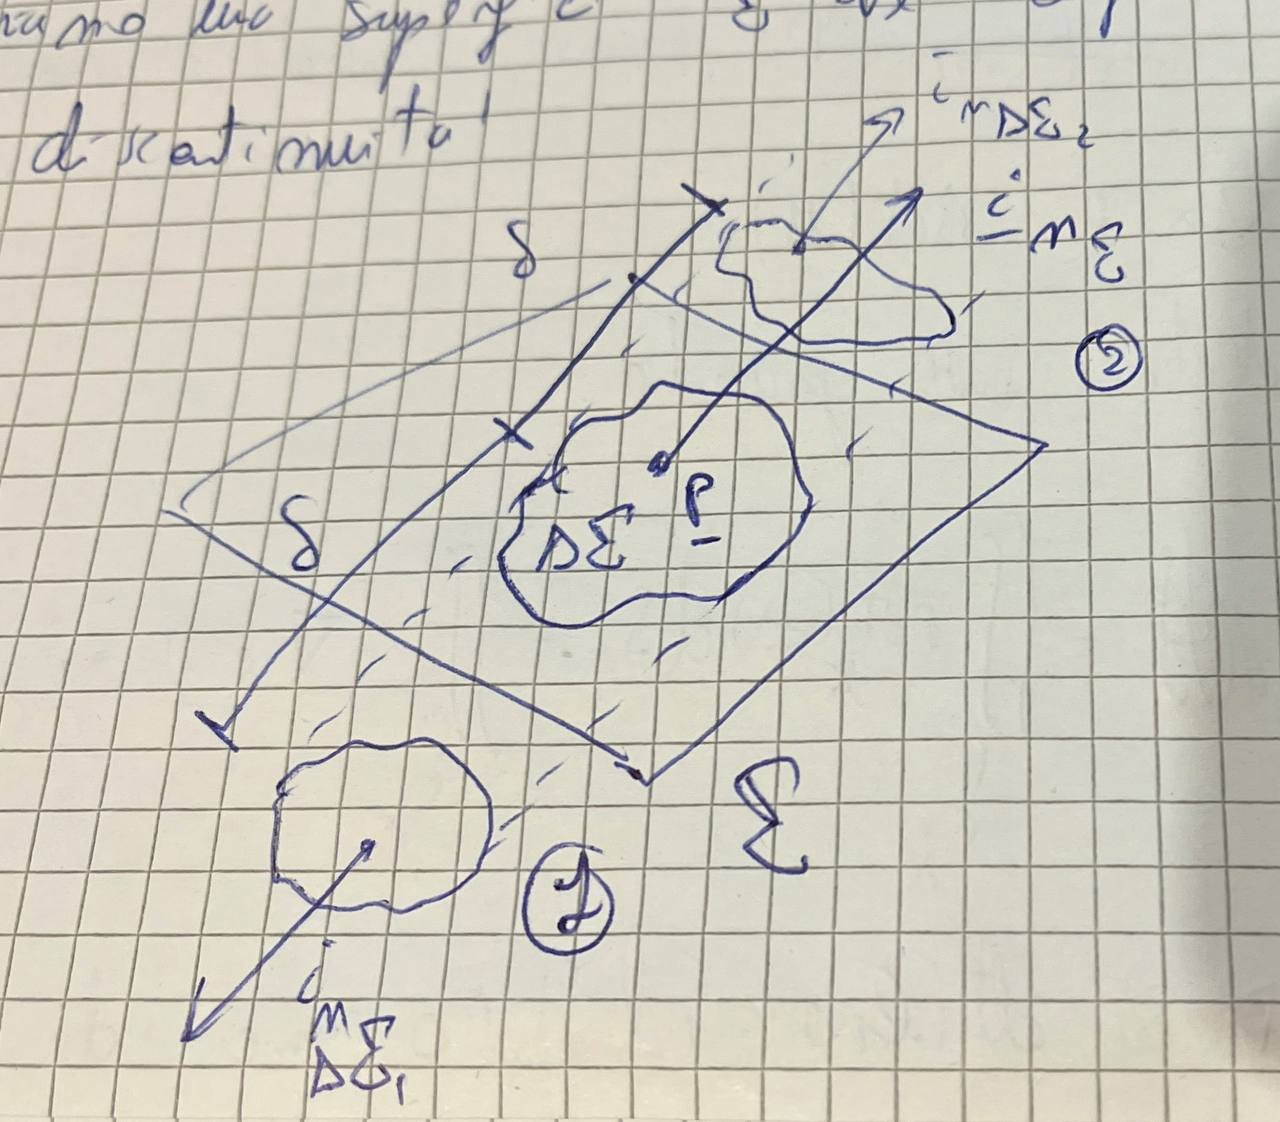
\includegraphics[width=0.5\linewidth]{img//Chapter_one/Chapt1img5.png}
            \caption{}
        \end{figure}
        Sulla $\Sigma$ consideriamo una superficie infinitesima $\Delta \Sigma$ e la facciamo traslare lungo la direzione della normale in entrambi i versi di una quantità $\delta$, generando il cilindroide di volume $V$, altezza $2 \delta$ e basi $\Delta \Sigma$. Chiamiamo la zona al di sotto della superficie "1" con la relativa base $\Delta \Sigma_{1}$ e normale opposta a quella di $\Delta \Sigma$, mentre quella di sopra sarà la superficie "2" con relativa base $\Delta \Sigma_{2}$ e normale con verso concorde a quella di $\Delta \Sigma$. La superficie laterale è $\Delta \Sigma_{l}$. \\ \\
        L'integrale di flusso attraverso il cilindroide si può scrivere come somma di tre contributi \footnote{Notare che non sono integrali chiusi perché tutti e tre formano una superficie chiusa, ma da soli sono semplicemente integrali di superfici aperte}:
        \begin{equation}
            \oiint_{\partial V} \underline{b} \cdot \underline{i_{n}} = \iint_{\Delta \Sigma_{1}} \underline{b} \cdot \underline{i}_{n} + \iint_{\Delta \Sigma_{2}} \underline{b} \cdot \underline{i}_{n} + \iint_{\Delta \Sigma_{1}} \underline{b} \cdot \underline{i}_{l}
        \end{equation} \\
        Dobbiamo far collassare il cilindroide al punto $P$. Facciamo il limite per $\delta \to 0$ ed analizziamo separatamente i tre contributi. Per la superficie laterale, la quantità:
        \begin{equation}
            \lim_{\delta \to 0} \iint_{\Delta \Sigma_{l}} \underline{b} \cdot \underline{i}_{n} dS
        \end{equation}
        \\ tende alla curva corrispondente al bordo di $\Delta \Sigma$. Per l'assoluta continuità dell'integrale\footnote{Integrando una funzione in un dominio perdendo un dimensione e tale funzione è regolare allora l'integrale va a zero} il contributo della superficie laterale è nullo. \\
        Per la superficie $\Delta \Sigma_{1}$, questa converge alla superficie $\Delta \Sigma$ come insieme di punti ma con normale opposta a quella di quest'ultima, dunque:
        \begin{equation}
            \iint_{\Delta \Sigma_{1}} \underline{b} \cdot \underline{i}_{n_{\Sigma}} dS \stackrel{\delta \to 0}{\to}  \iint_{\Delta \Sigma} \underline{b} \cdot (- \underline{i}_{n_{\Sigma}} )dS
        \end{equation} \\
        In modo analogo, $\Delta\Sigma_{2} \stackrel{ \delta \to 0}{\to} \Delta \Sigma$ ottenendo:
        \begin{equation}
            \iint_{\Delta \Sigma_{2}} \underline{b} \cdot \underline{i}_{n_{\Sigma}} dS \stackrel{\delta \to 0}{\to}  \iint_{\Delta \Sigma} \underline{b} \cdot - \underline{i}_{n_{\Sigma}} dS
        \end{equation}
        Tenendo conto del fatto che il campo $\underline{b}$ avrà espressioni generalmente diverse in "1" e "2", ovvero $\underline{b}_{1}$ e $\underline{b}_{2}$, scriviamo in definitiva:
        \begin{equation}
            \lim_{\delta \to 0} \iint_{\Delta \Sigma_{1}} \underline{b} \cdot \underline{i}_{n} + \iint_{\Delta \Sigma_{2}} \underline{b} \cdot \underline{i}_{n} + \iint_{\Delta \Sigma_{1}} \underline{b} \cdot \underline{i}_{l} = \iint_{\Delta \Sigma} (\underline{b}_{2}-\underline{b}_{1}) \cdot \underline{i}_{n}dS = 0
        \end{equation}
        Possiamo affermare che l'argomento di quest'integrale è nullo grazie al \textbf{teorema della localizzazione}, il quale afferma che se una funzione $f(x)$ viene integrata su un dominio $I$ arbitrario e per ogni $I$ il suo integrale ha valore nullo, allora $f(x) = 0$ quasi ovunque. \\
        Nel nostro caso $\Delta \Sigma$ è stata scelta in modo arbitrario e dunque possiamo scrivere:
        \begin{equation}
        \label{eqn:condizione_raccordo4}
            (\underline{b}_{2}-\underline{b}_{1}) \cdot \underline{i}_{n_{\Sigma}} = 0 \quad \quad \forall \Delta \Sigma
        \end{equation}
        La (\ref{eqn:condizione_raccordo4}) è la \textit{quarta equazione di raccordo} che va utilizzata in presenza di discontinuità per le quali non è possibile utilizzare la quarta legge di Maxwell in forma locale. È importante notare come la (\ref{eqn:condizione_raccordo4}) derivi direttamente dalle equazioni di Maxwell e sottolinea come esse debbano valere anche in presenza di discontinuità. In questo caso, la legge che abbiamo appena ricavato richiede che le componenti normali\footnote{sono infatte moltiplicate per il versore normale} del campo di induzione magnetica $\underline{b}$ si conservino. \\
        Un ultima osservazione va fatta sulla drammatica differenza di significato fra le condizioni al \textit{contorno} e quelle di \textit{raccordo}: le prime danno un'informazione numerica, cioè quanto devono valere i campi alla frontiera, mentre quelle di raccordo danno informazioni circa la relazione fra i campi delle due superfici, come nel caso appena trattato fra $\underline{b}_{1}$ e $\underline{b}_{2}$. \\ \\
        Passiamo ora alla terza equazion di raccordo. Utilizziamo la stessa figura di prima ma stavolta l'equazione da considerare è:
        \begin{equation}
            \oiint_{\partial V} \underline{d} \cdot \underline{i}_{n} dS = q(V, t)
        \end{equation}
        che è più complessa rispetto alla quarta per la presenza di un termine non per forza nullo a secondo membro. \newpage Come prima scriviamo:
        \begin{equation}
            \iint_{\Delta \Sigma_{1}} \underline{d} \cdot \underline{i}_{n} dS + \iint_{\Delta \Sigma_{2}} \underline{d} \cdot \underline{i}_{n} dS + \iint_{\Delta \Sigma_{l}} \underline{d} \cdot \underline{i}_{n}  dS= q(V,t) 
        \end{equation}
        I termini del primo membro con lo stesso procedimento di prima danno, al limite per $\delta \to 0$:
        \begin{equation}
            \iint_{\Delta \Sigma} (\underline{e}_{2}-\underline{e}_{1}) \cdot \underline{i}_{n} dS
        \end{equation}
        ma dove converge $\displaystyle \lim_{\delta \to 0} q(V,t)$? Consideriamo una superficie $\Sigma$ con della carica distribuita su uno strato di un certo spessore:
        \begin{figure}[h!]
            \centering
            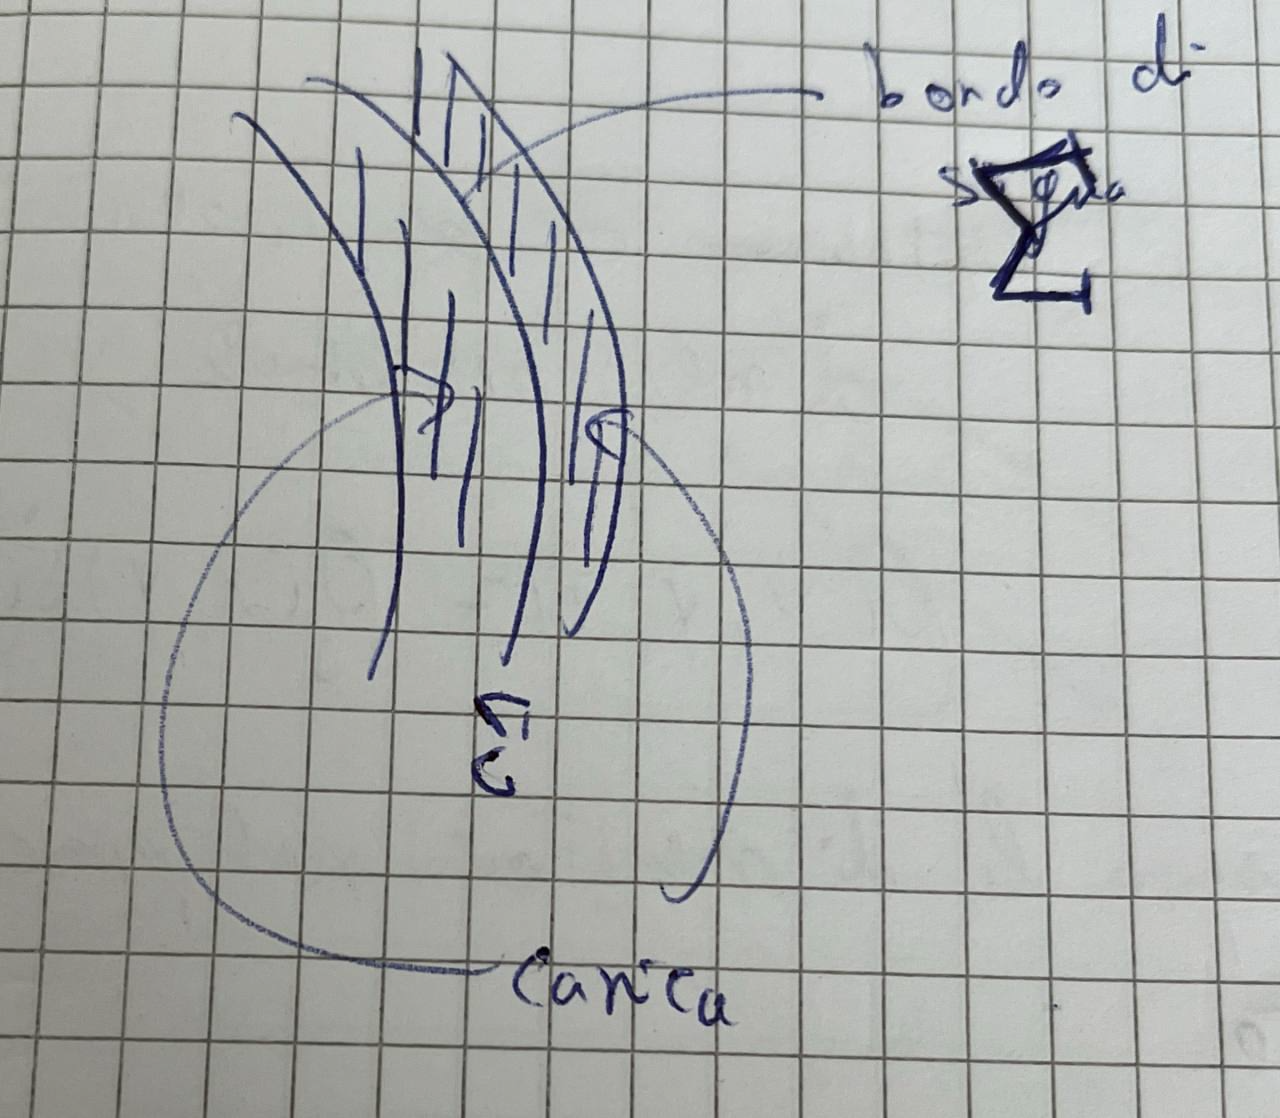
\includegraphics[width=0.5\linewidth]{img//Chapter_one/chapt1img6.png}
            \caption{}
        \end{figure}
        Se tale spessore è trascurabile rispetto alle altre dimensioni in gioco, possiamo dire in modo approssimato che la carica ivi contenuta sia totalmente sulla superficie $\Sigma$, cioè stiamo passando da una densità di carica volumica ad una superficiale. Teniamo conto infatti che:
        \begin{equation}
            q(V,t) = \iiint_{V} \rho dV
        \end{equation}
        Ma se la densità $\rho(x,y,z)$ è distribuita su una superficie\footnote{che supponiamo piana perché tutte le superfici se non le vedi come un nerd sono piane}, allora deve essere non nulla soltanto in quei punti che hanno come coordinata la $z_{0}$ fissata del piano:
        \begin{figure}[h!]
            \centering
            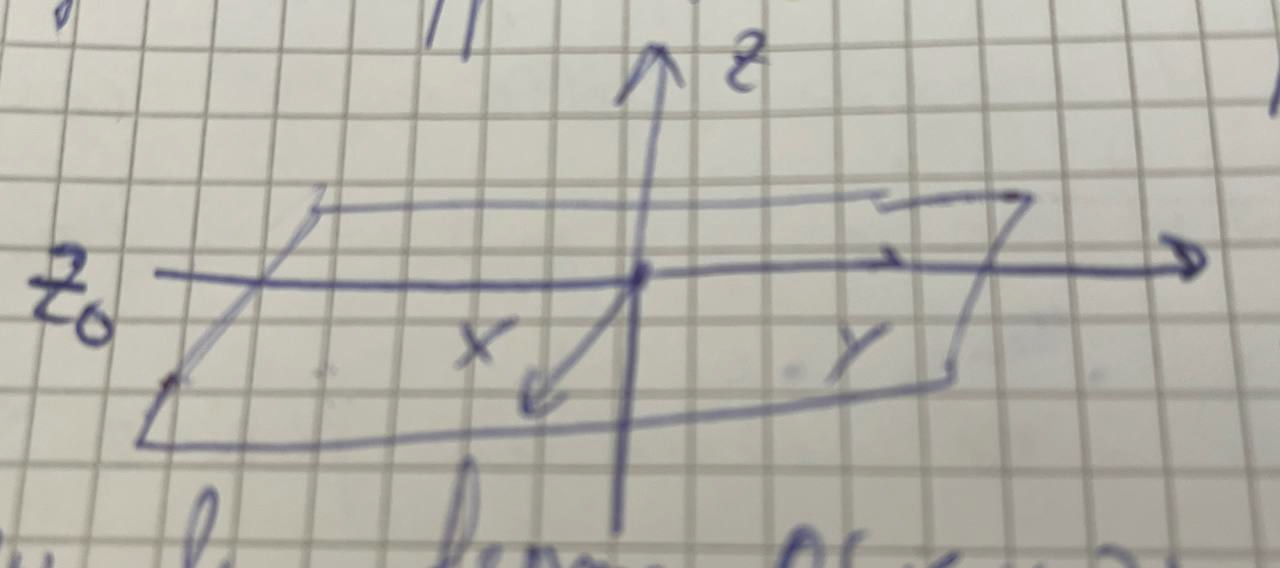
\includegraphics[width=0.36\linewidth]{img/Chapter_one/chapt1img7.png}
            \caption{}
        \end{figure}
        \newpage
        allora $\rho(x,y,z)$ dovrà avere una forma del genere:
        \begin{equation}
        \label{eqn:densità_carica_sup}
            \rho (x,y,z) = \rho_{S}(x,y)\delta(z)
        \end{equation}
        dove $\rho_{S}(x,y)$ è la \textbf{densità superficiale di carica} che ha dimensioni $C/m^{2}$. È bene notare che affinché la (\ref{eqn:densità_carica_sup}) abbia dimensionalmente senso, la $\delta(z)$ deve avere le dimensioni di un inverso di una lunghezza. La delta infatti è tale per cui:
        \begin{equation}
            \int ^{\chi} _{-\chi} \delta(\chi) d\chi = 1
        \end{equation}
        qualunque sia $\chi$. Poiché il risultato è un numero adimensionale, la delta deve avere le dimensioni inverse di $\Delta \chi$. Nel nostro caso, l'integrale fatto lungo la componente $z$, che ha le dimensioni di una lunghezza, deve ritornare $1$ per la proprietà di $\delta (z)$, che quindi è omogenea ad $\displaystyle \frac{1}{m}$.
        In definitiva, possiamo scrivere:
        \begin{equation}
            \iint_{\Delta \Sigma} [(\underline{d}_{2}-\underline{d}_{1}) \cdot \underline{i}_{n} -\rho_{s}]dS = 0
        \end{equation}
        Applicando come prima il teorema della localizzazione otteniamo la \textit{terza equazione al raccordo}:
        \begin{equation}
        \label{eqn:cond_raccordo_3}
            (\underline{d}_{2}-\underline{d}_{1}) \cdot \underline{i}_{n} = \rho_{s}
        \end{equation} \\
        La (\ref{eqn:cond_raccordo_3}) asserisce che la componete normale del campo di induzione magnetica nel passaggio da un mezzo all'altro, in presenza di accumuli di carica superficiali con densità di carica $\rho_{s}$, debbano variare proprio di $\rho_{s}$.
        \newpage
        \subsection{Seconda e prima legge di Maxwell}
        Passiamo ora alla II equazione di Maxwell.
        \begin{figure}[h!]
            \centering
            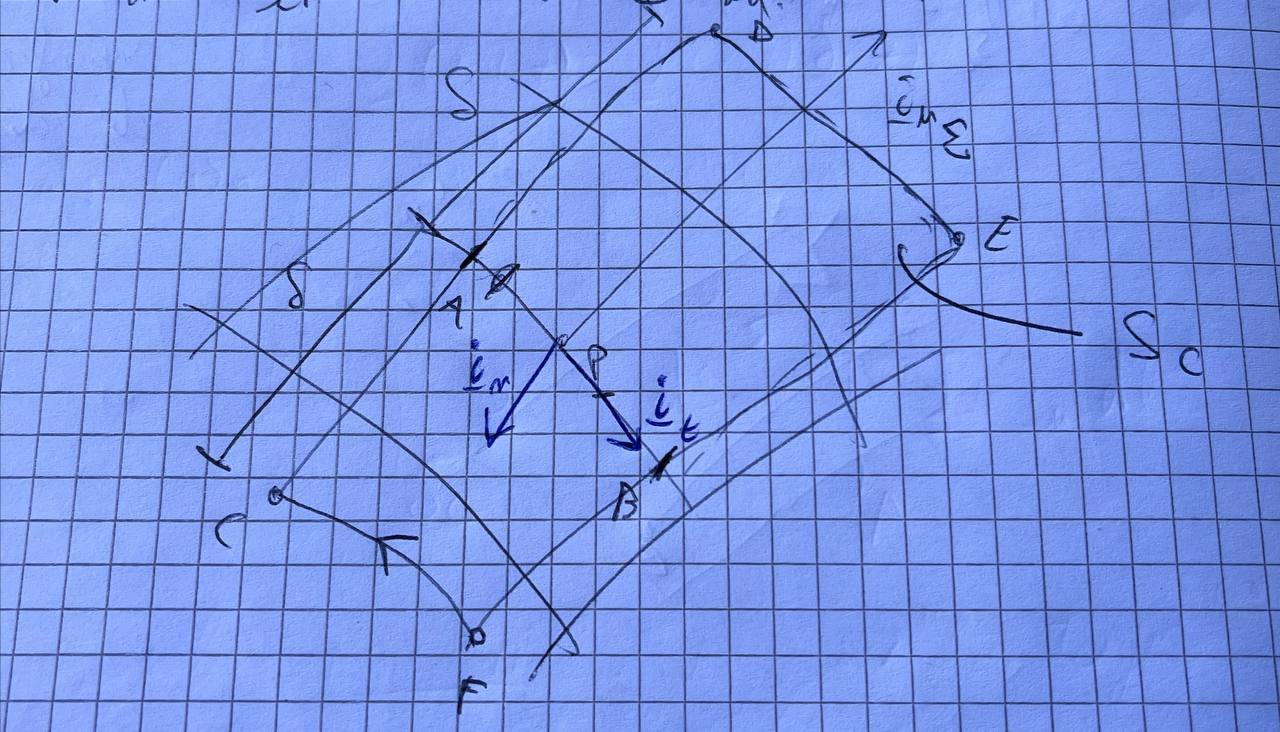
\includegraphics[width=0.75\linewidth]{img//Chapter_one/chapt1img5age.png}
            \caption{}
        \end{figure}
        Consideriamo una superficie $\Sigma$ e scegliamo arbitrariamente uno del fascio di piani generato dalla normale a $\Sigma$. Tale piano individua sulla superficie $\Sigma$ la curva $AB$. A partire da AB efiniamo il rettangoloide $CDEF$ dove $DE$ e $CF$ sono distanti $\delta$ rispetto ad $AB$. Orientiamo la curva $CFDE$, che chiamiano $\mathcal{C}$ con tangente $\underline{i}_{t}$, la quale è il bordo della superficie $S_{\mathcal{C}}$ con normale $\underline{i}_{n}$, corrispondente proprio al rettangoloide individuato da $CDEF$. \\
        La circuitazione lungo $\mathcal{C}$ può essere scritta come:
        \begin{equation}
            \oint_{\mathcal C} \underline{h} \cdot \underline{i}_{l} dl = \int_{C} ^{D} \underline{h} \cdot \underline{i}_{l}dl + \int_{D} ^{E} \underline{h} \cdot \underline{i}_{l}dl +\int_{E} ^{F} \underline{h} \cdot \underline{i}_{l}dl +\int_{C} ^{F} \underline{h} \cdot \underline{i}_{l}dl  
        \end{equation}
        Vediamo dove convergono questi termini per $\delta \to 0$. L'integrale di linea lungo $DC$ va a zero, perché perde una dimensione\footnote{in quanto $DC$ sta collassando al punto $A$}. Lo stesso discorso va fatto per quello lungo $EF$.\\
        Per $\delta \to 0$ la curva $DE$ diventa pari ad $AB$ con versore concorde\footnote{orientando la curva in senso orario} a quello tangente ad essa. Il campo nella zona superiore, dove c'è $DE$ per intenderci, ha valore $\underline{h}_{2}$ e quindi:
        \begin{equation}
            \int_{D} ^{E} \underline{h} \cdot \underline{i}_{l}dl \stackrel{\delta \to 0}{\to} \int_{A} ^{B} \underline{h}_{2} \cdot \underline{i}_{t} dl
        \end{equation}
        In modo analogo:
        \begin{equation}
            \int_{C} ^{F} \underline{h} \cdot \underline{i}_{l}dl \stackrel{\delta \to 0}{\to} \int_{A} ^{B} \underline{h}_{1} \cdot (-\underline{i}_{t}) dl
        \end{equation}
        \\ A secondo membro, il contributo associato al campo induzione elettrica è:
        \begin{equation}
            \lim_{\delta \to 0} \frac{\partial}{ \partial t} \iint_{S_{\mathcal{C}}} \underline{d} \cdot \underline{i}_{n}dS = \lim_{\delta \to 0} \iint_{S_{\mathcal{C}}} \frac{\partial}{\partial t} \underline{d} \cdot \underline{i}_{n} dS = 0
        \end{equation}
        questo perché $S_{\mathcal{C}}$ degenera in $AB$. Per il termine di corrente scriviamo:
        \begin{equation}
            \lim_{\delta \to 0} i(\underline{S}_{\mathcal{C}}, t) = \lim_{\delta \to 0} \iint_{S_{\mathcal{C}}} \underline{j} \cdot \underline{i}_{n}dS
        \end{equation}
        Sembrerebbe annullarsi perchè $S_{\mathcal{C}}$ tende al punto! Ma se ammettiamo che possano esserci degli accumuli di densità di corrente superficiali $\underline{j}_{S}$ tali per cui:
        \begin{equation}
            \underline{j}(x,y,z) = \underline{j}_{S}(x,y) \delta (z)
        \end{equation}
        In tal caso quel limite di prima non si annulla, perché l'integrale su $S_{\mathcal{C}}$ da contributo unitario lungo la direzione $z$ per le proprietà della delta:
        \begin{equation}
            \lim_{\delta \to 0} \iint_{S_{\mathcal{C}}} \underline{j}_{S} \cdot \underline{i}_{n}dl
        \end{equation}
        Notiamo che l'integrale di linea viene fatto sulla \textit{tangente} ad $AB$ $\underline{i}_{n}$ e non sulla tangente, questo perché l'informazione che interessa a noi è "quanta corrente sta uscendo per la superficie per il limite per $\delta \to 0$?". \\
        Alla luce di quanto detto possiamo scrivere, per $\delta \to 0$:
        \begin{align}
            \int_{A} ^{B} \underline{h}_{2} \cdot \underline{i}_{t}dl - \int_{A} ^{B} \underline{h}_{1} \cdot \underline{i}_{t}dl = \int_{A} ^{B} \underline{j}_{S} \cdot \underline{i}_{n} dl \\ \implies
            \int_{A} ^{B} [(\underline{h_{2}-\underline{h}_{1}}\cdot \underline{i}_{t})-\underline{j}_{S}\cdot \underline{i}_{n}]dl = 0
        \end{align}
        Poiché $AB$ è una curva arbitraria, vale il teorema della localizzazione e dunque si può scrivere:
        \begin{equation}
            (\underline{h}_{2}-\underline{h}_{1}) \cdot \underline{i}_{t} = \underline{j}_{S} \cdot \underline{i}_{n}
        \end{equation}
        Ma la controparte differenziale\footnote{$\nabla \times \underline{h} = \underline{j} + \frac{\partial}{\partial} \underline{d}$} è un'equazione vettoriale, mentre questa è una relazione scalare. La $\underline{i}_{n}$ è ortogonale ad $S_{C}$ e tangente a $\Sigma$, mentre $\underline{i}_{t}$ è tangente a $\Sigma$ ed $\underline{i}_{n\Sigma}$\footnote{la normale di $\Sigma$} ortogonale a $\Sigma$. Allora $\underline{i}_{t}, \underline{i}_{n}, \underline{i}_{n\Sigma}$ e quindi si può scrivere:
        \begin{equation}
            i_{t} = \underline{i}_{n} \times \underline{i}_{n\Sigma}
        \end{equation}
        per cui
        \begin{equation}
            (\underline{h}_{2}-\underline{h}_{1}) \cdot \underline{i}_{n} \times \underline{i}_{n\Sigma} = \underline{j}_{S} \cdot \underline{i}_{n}
        \end{equation}
        Applicando le proprietà del prodotto misto\footnote{un prodotto misto è del tipo $a \times b \cdot c$ e rimane invariato per permutazioni cicliche degli indici, per le quali $a \times b \cdot c = c \times a \cdot b = b \times c \cdot a$}:
        \begin{equation}
            \underline{i}_{n} \cdot \underline{i}_{n \Sigma} \times (\underline{h}_{2}-\underline{h}_{2}) = \underline{j}_{S} \cdot \underline{i}_{n}
        \end{equation}
        Se questa relazione vale per ogni $\underline{i}_{n}$, e cioè per ogni componente del versore normale ad $S_{\mathcal{C}}$, allora possiamo cancellarlo. La scelta dei piani del fascio è arbitraria, quindi $\underline{i}_{n}$ può variare rimanendo tangente a $\Sigma$. Allora per quel che riguarda la componente tangente a $\Sigma$ i due vettori sono uguali. Ci manca la direzione normale, ma la componente normale di $\underline{i}_{n\Sigma} \cdot (\underline{h}_{2}-\underline{h}_{1})$ è:
        \begin{equation}
            \underline{i}_{n\Sigma} \cdot \underline{i}_{n\Sigma} \cdot (\underline{h}_{2}-\underline{h}_{1}) = 0
        \end{equation}
        per le proprietà del prodotto misto.\footnote{$a \cdot a \times b = b \cdot (a \times a) = 0$ perché ogni vettore è parallelo a se stesso dunque il prodotto vettoriale fra due vettori identici è nullo} Inoltre $\underline{j}_{S} \cdot \underline{i}_{n \Sigma} = 0$ perché $\underline{j}_{S}$ ha normale tangente a $\Sigma$.\\
        In definitiva si può scrivere la \textit{seconda equazione al raccordo}:
        \begin{equation}
            \label{eqn:equazione_raccordo2}
            i_{n \Sigma} \times (\underline{h}_{2}-\underline{h}_{1}) = \underline{j}_{S}
        \end{equation}
        Notiamo che questa relazione non esprime però le condizioni al raccordo delle componenti normali del campo magnetico, bensì a quelle tangenti ruotate di $\frac{\pi}{2}$. Per vederlo, consideriamo una superficie $\Sigma$ con normale $\underline{i}_{n}$:
        \begin{figure}[h!]
            \centering
            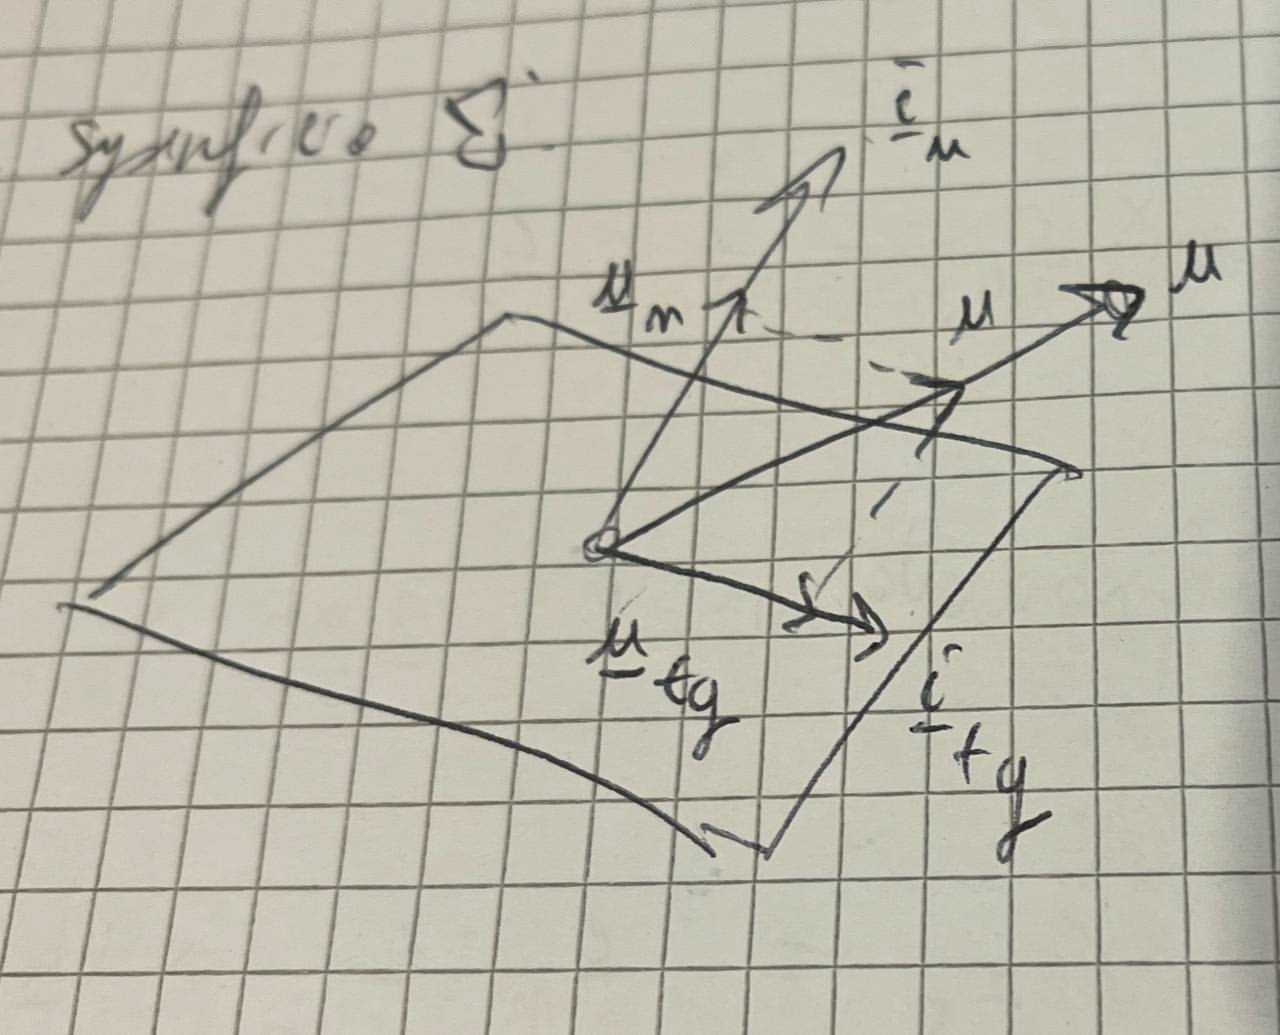
\includegraphics[width=0.60\linewidth]{img/Chapter_one/Chapt1img7.png}
        \end{figure}
        Per la componente normale del generico vettore $\underline{u}$ possiamo scrivere:
        \begin{equation}
            \underline{u}_{n} = (\underline{u} \cdot \underline{i}_{n \Sigma}) \underline{i}_{n \Sigma}
        \end{equation}
        mentre per quella tangenziale, in assenza di versore tangenziale, possiamo prendere il vettore e sottrargli la componente normale:
        \begin{equation}
            \underline{u}_{tg} = (\underline{u}-\underline{u}_{n}) = \underline{u} \cdot (\underline{u}-\underline{i}_{n \Sigma}) i_{n \Sigma}
        \end{equation}
        il quale è un doppio prodotto vettoriale\footnote{$(\underline{a} \times \underline{b}) \times c = (\underline{a} \cdot \underline{c}) \underline{b} - (\underline{b} \cdot \underline{c})\underline{a}$} che si può riscrivere come:
        \begin{equation}
        \label{eqn:componente_tangente}
            (\underline{i}_{n \Sigma} \times \underline{u}) \times \underline{i}_{n \Sigma}
        \end{equation}
        che è l'espressione della componente tangente di $\underline{u}$. Se confrontiamo la (\ref{eqn:componente_tangente}) con la $(\ref{eqn:equazione_raccordo2})$ ci si rende conto che non combaciano in termini di forma. Per ottenere infatti la componente rigorosamente tangente del campo magnetico dovremmo moltiplicare vettorialmente per $\underline{i}_{n}$, perché $\underline{i}_{t} = \underline{i}_{n} \times \underline{i}_{n\Sigma}$. \\
        Per la prima legge di Maxwell abbiamo un espressione analoga:
        \begin{equation}
            \underline{i}_{n \Sigma} \times (\underline{e}_{2}-\underline{e}_{1}) = 0
        \end{equation}
        cioè le componenti tangenti\footnote{ruotate di novanta gradi} del campo elettrico si conservano, perché nella prima legge non c'è dipendenza da termini che esprimono densità superficiali.\\ Ricapitolando:
        \begin{equation}
        \begin{cases}
            \underline{i}_{n} \times (\underline{e}_{2} - \underline{e}_{1}) = 0 \\
            i_{n \Sigma} \times (\underline{h}_{2}-\underline{h}_{1}) = \underline{j}_{S} \\
            \underline{i}_{n} \cdot (\underline{d}_{2} - \underline{d}_{1}) = \rho_{S} \\
            \underline{i}_{n} \cdot (\underline{b}_{2}-\underline{b}_{1}) = 0
        \end{cases}
        \end{equation}
    \section{L'equazione di continuità}
        Dimostriamo che l'equazione di continuità è contenuta in quelle di Maxwell, non aggiungendo de facto contenuto informativo. La sua forma integrale è:
        \begin{equation}
            -\frac{\partial}{\partial t} q(V, t) = i(\partial \underline{V}, t)
        \end{equation}
        che riscritta è
        \begin{equation}
            -\frac{\partial}{\partial t} \iiint_{V} \rho dV = \oiint_{\partial V} \underline{j} \cdot \underline{i}_{n} dV 
        \end{equation}
        Sotto l'ipotesi che si possa portare la derivata sotto il segno d'integrale ed applicando il teorema di Gauss a secondo membro, scriviamo:
        \begin{equation}
            \iiint_{V} [\frac{\partial}{\partial t} \rho + \nabla \cdot \underline{j}]dV = 0
        \end{equation}
        Poiché l'equazione di continuità vale qualunque sia $V$, applichiamo il teorema di localizzazione per ricavare l'espressione differenziale:
        \begin{equation}
        \label{eqn:eq_continuità_diff}
            \frac{\partial}{\partial t} \rho + \nabla \cdot \underline{j} = 0
        \end{equation}
        La (\ref{eqn:eq_continuità_diff}) è ricavabile applicandol'operatore divergenza ad ambo membri della terza equazione di Maxwell:
        \begin{equation}
            \nabla \cdot \nabla \times \underline{h} = \nabla \cdot (\frac{\partial}{\partial t} \underline{d} + \underline{j})
        \end{equation}
        Se $\underline{d}$ è differenziabile $\nabla \cdot \frac{\partial}{\partial t} \underline{d} = \frac{\partial}{\partial t} \nabla \cdot \underline{d}$. Inoltre, in virtù del fatto che la divergenza del rotore è nulla si ottiene:
        \begin{equation}
            \frac{\partial}{\partial t} \nabla \cdot \underline{d} + \nabla \cdot \underline{j} = \frac{\partial}{\partial t} \rho + \nabla \cdot \underline{j} = 0
        \end{equation}
        QED. 
        \section{Le relazioni costitutive}
            Le relazioni costitutive legano $\underline{e}$ ed $\underline{h}$, grandezze d'ingresso, a $\underline{d},\underline{b}$ e $\underline{j}$, grandezze di uscita. Le corrispondenze ingresso-uscita sono:
            \begin{align}
                \underline{d} (\underline{r}, t) = \hat{D}[\underline{e}(\underline{r}, t), \underline{h}(\underline{r}, t)] \\
                \underline{b} (\underline{r}, t) = \hat{B}[\underline{e}(\underline{r}, t), \underline{h}(\underline{r}, t)] \\
                \underline{j} (\underline{r}, t) = \hat{J}[\underline{e}(\underline{r}, t), \underline{h}(\underline{r}, t)] 
            \end{align}
            le quali non sono corrispondenze numeriche, perché bisogna conoscere \underline{e} ed $\underline{h}$ in ogni punto dello spazio ed in ogni istante di tempo precedente a quello corrente. Al contrario, sono \textbf{corrispondenze operatoriali} e sono tali da prelevare in ingresso funzioni e restituire in uscita funzioni. \\
            Tutte le relazioni costitutive devono soddisfare le proprietà di \textit{causalità, continuità e stabilità BIBO}. Analizziamo nel dettaglio tutte e tre. \\ \\
            La causalità si divide in \textbf{debole} e \textbf{forte}. La causalità debole richiede che l'effetto non deve precedere la causa. Non ci sono relazioni causa-effetto istantanee, allora l'effetto è necessariamente successivo alla causa. Se la causa avviene nella posizione $\underline{r}$ e l'effetto nella posizione $\underline{r}'$, ci sarà un ritardo minimo pari a:
            \begin{equation}
                \Delta t_{min} = \frac{|\underline{r}-\underline{r}'|}{c}
            \end{equation}
            In altre parole, se $t$ è l'istante in cui si manifesta la causa e $t'$ quello in cui si manifesta l'effetto, deve risultare:
            \begin{equation}
            \label{eqn:caus_forte}
                |t-t'| \geq \Delta t_{min}
            \end{equation}
            La causalità forte vale se la (\ref{eqn:caus_forte}) è verificata.\footnote{Ma non se è del tipo strettamente minore, ovvero se $|t-t'|< \Delta t_{min}$}\\
            La causalità debole\footnote{anche lei non vale se è del tipo strettamente minore} è soddisfatta se:
            \begin{equation}
                t-t' \geq 0
            \end{equation}
            Ne consegue che la causalità forte include quella causale ma non viceversa. \\ \\
            La causalità richieda che se varia la causa in maniera sempre minore fino ad annullare la sua variazione, allora si deve comportare di conseguenza anche l'uscita. La stabilità BIBO (Bounded Input Bounded Output) richiede che ad ingresso finito ci sia uscita finita. \\ \\
            Le relazioni costitutive vanno studiare per \textit{classi di mezzi}, in modo tale da studiare un caso valido per ogni membro di una data classe. Le proprietà da verificare (o no) sono:
            \begin{itemize}
                \item Linearità
                \item Non dispersività spaziale e temporale
                \item Omogeneietà spaziale e temporale\footnote{quest'ultima altresì detta stazionarietà}
                \item Isotropia
            \end{itemize}
            \subsection{Linearità}
            Noi ipotizziamo che $\underline{d}$ dipenda solo da $\underline{e}$, $\underline{b}$ solo da $\underline{h}$ e $\underline{j}$ solo da $\underline{e}$, assunzione che vale per una grande quantità di mezzi quando non sono in movimento. \\
            Un mezzo è \textbf{lineare} se risulta per due ingressi $\underline{e}_{1}$ ed $\underline{e}_{2}$ 
            \begin{equation}
            \hat{D}[c_{1}\underline{e}_{1}+c_{2}\underline{e}_{2}] = c_{1} \hat{D}[\underline{e}_{1}]+c_{2}\hat{D}[\underline{e}_{2}]
            \end{equation}
            La relazione costitutiva per $\underline{d}$\footnote{stesso discorso per $\underline{b}$ e $\underline{j}$} ha la forma:
            \begin{equation}
            \label{eqn:eq_costitutivaTemplate}
                \underline{d}(\underline{r},t) = \iiiint_{\mathbb{R}^{4}} d\underline{r}' dt' \underline{\underline{g}}(\underline{r}. \underline{r}', t, t') \underline{e}(\underline{r}', t')
            \end{equation}
            dove $\underline{\underline{g}}$ è una matrice detta \textbf{funzione diadica di Green}. È intuibile capire il perché della (\ref{eqn:eq_continuità_diff}). Sia $(\underline{r}', t')$ la posizione di una certa causa che ha effetto in $(\underline{r}, t)$. La generica relazione causa-effetto sarà del tipo:
            \begin{equation}
                \underline{d}(\underline{r}, t) = \underline{\underline{g}} \cdot\underline{e}(\underline{r}, t)
            \end{equation}
            Ma se ci sono cause per ogni punto dello spazio ed il sistema è lineare, per tenerle in conto tutte dobbiamo sommare su tutto lo spazio e dunque si ottiene la (\ref{eqn:eq_costitutivaTemplate}). Tuttavia, la (\ref{eqn:eq_costitutivaTemplate}) integra nel tempo da $-\infty$ a $+\infty$, ma i sistemi che consideriamo devono essere causali. Ciò significa che andrebbe riscritta come:
            \begin{equation}
                \underline{d}(\underline{r},t) = \iiint_{\mathbb{R}^{3}} d\underline{r}' \int_{-\infty} ^{t} dt' \underline{\underline{g}}(\underline{r}. \underline{r}', t, t') \underline{e}(\underline{r}', t')
            \end{equation}
            La (\ref{eqn:eq_costitutivaTemplate}) può essere comunque utilizzata\footnote{E noi questa utilizzeremo} se imponiamo che la funzione di Green si annulli per $t'>t$. 
            \subsection{Non dispersività}
            Un mezzo è \textbf{temporalmente non dispersivo} se l'effetto in un istante dipende da cause unicamente in quell'istante, cioè se il mezzo è "senza memoria". La \textbf{non dispersività spaziale} è definita in modo analogo e richiede che il l'effetto dipenda soltanto dalla causa nello stesso punto e non da altri. \\
            Se ora consideriamo un sistema lineare e non dispersivo nello spazio, si può scrivere:
            \begin{equation}
                \underline{d}(\underline{r},t) = \int_{\mathbb{R}} dt' \underline{\underline{g}'}(\underline{r}, t, t') \underline{e}(\underline{r}, t)
            \end{equation}
            perché $\underline{r}$ è fissato per la non dispersività e dunque possiamo definire una funzione di Green $\underline{\underline{g}'}$ tale per cui:
            \begin{equation}
                \underline{\underline{g}}(\underline{r}, \underline{r}', t, t') = \underline{\underline{g}}' (\underline{r}, t, t')\delta(\underline{r}-\underline{r}')
            \end{equation}
            \\ Ipotizziamo ora che valga la non dispersività temporale. La relazione costitutiva sarà:
            \begin{equation}
                \underline{d} (\underline{r}, t) = \iiint_{\mathbb{R}} d \underline{r}' \underline{\underline{g}}'' (\underline{r}, \underline{r}', t) \underline{e}(\underline{r},t)
            \end{equation}
            dove $\underline{\underline{g}} (\underline{r}, \underline{r}', t, t') = \underline{\underline{g}}''(\underline{r}, \underline{r}', t, t') \delta(t-t')$. \\
            La non dispersività temporale implica la non dispersività spaziale, perché le cause in altri punti da quello corrente si propagano in tempi non nulli, ma per la non dispersività temporale la causa dipende solo dall'istante corrente e non da istanti precedenti.
            Poiché la dispersività temporale implica quella spaziale, sotto tale ipotesi la (\ref{eqn:eq_costitutivaTemplate}) si può scrivere come:
            \begin{equation}
                \underline{d} (\underline{r}, t) = \underline{\underline{g}}''' (\underline{r}, t) \underline{e}(\underline{r}, t)
            \end{equation}
            con $\underline{\underline{g}} (\underline{r}, \underline{r}', t, t') = \underline{\underline{g}}'''(\underline{r}, t) \delta(\underline{r}-\underline{r}')\delta(t-t')$. \\
            Per fare una preview di quello che sarà approfondito dopo, la funzione di Green in nel caso non dispersivo è la permettività elettrica del mezzo:
            \begin{equation}
                \underline{d}(\underline{r},t) = \underline{\underline{\varepsilon}} (\underline{r}, t)\underline{e}(\underline{r}, t)
            \end{equation}
            \subsection{Omogeneità}
            Un mezzo si dice \textbf{omogeneo nel tempo}, o anche \textbf{stazionario}, se risulta $\forall t_{0}$ e $\forall \underline{e}$:
            \begin{equation}
                \hat{D} [\ \hat{\tau}_{t_{0}}[\underline{e}(\underline{r}, t)] \ ] = \hat{\tau}_{t_{0}}[\ \hat{D}[\underline{e}(\underline{r},t)]\ ]
            \end{equation}
            dove $\hat{\tau}_{t_{0}} :\hat{\tau}_{t_{0}} [\ \underline{e}(\underline{r},t) \ ] = \underline{e}(\underline{r}, t+t_{0})$ è l'operatore di traslazione temporale di valore $t_{0}$. \\ 
            In altri termini, l'omogeneità temporale richiede che l'uscita sia invariante per traslazione temporale, che è l'equivalente dell'affermare che gli operatori $\hat{D}$ e $\hat{\tau}$ commutano\footnote{Cioè l'ordine con cui vengono applicati è irrilevante, ma ovviamente è un caso speciale e non è sempre così}. \\
            Un mezzo si dice \textbf{omogeneo nello spazio} se $\forall r_{0}, \underline{e}$:
            \begin{equation}
                \hat{D} [\ \hat{\tau}_{r_{0}}[\underline{e}(\underline{r}, t)] \ ] = \hat{\tau}_{r_{0}}[\ \hat{D}[\underline{e}(\underline{r},t)]\ ]
            \end{equation}
            cioè se $\hat{D}$ e $\hat{\tau}_{r_{0}}$\footnote{l'operatore traslazione di valore $\underline{r_{0}}$ nello spazio} commutano. \\
            Nel caso in cui c'è omogeneità spaziale la relazione costitutiva generica si scrive\footnote{Nel caso semplificativo di considerare un sistema lineare con relazione ingresso-uscita non vettoriale}:
            \begin{equation}
                y(t) = \int_{\mathbb{R}} dt' g(t, t') x(t')
            \end{equation}
            Ci si chiede allora cosa succede se supponiamo che il mezzo goda anche della stazionarietà (omogeneità temporale). \\ Sia $y_{t_{0}}$ è l'uscita ottenuta dall'ingresso traslato di $t_{0}$ e $y(t-t_{0})$ l'uscita traslata di $t_{0}$:
            \begin{equation}
                y_{t_{0}}(t) = \int_{\mathbb{R}} dt' g(t, t') x(t'-t_{0})
            \end{equation}
            \begin{equation}
                y(t-t_{0}) = \int_{\mathbb{R}} dt' g(t-t_{0},t') x(t')
            \end{equation}
            Queste due termini sono uguali per la stazionarietà:
            \begin{equation}
                \int_{\mathbb{R}} dt' g(t, t') x(t'-t_{0}) = \int_{\mathbb{R}} dt' g(t-t_{0},t') x(t')
            \end{equation}
            Effettuando un cambio di variabile $t'' = t'-t_0$ si ottiene:
            \begin{equation}
                \int_{\mathbb{R}} dt' g(t, t''+t_{0}) x(t'') = \int_{\mathbb{R}} dt' g(t-t_{0},t') x(t')
            \end{equation}
            La variabile di integrazione è "muta", cioè il nome è irrilevante e $t'$ può essere benissimo uguale a $t''$ ai fine dell'integrale. Allora si può raccogliere tutto sotto un unico integrale:
            \begin{equation}
                \int_{\mathbb{R}} dt'[x(t')[g(t, t'+t_{0})-g(t-t_{0}, t')]] = 0
            \end{equation}
            Poiché questa relazione deve valere $\forall x(t)$ per ipotesi di stazionarietà spaziale, si può scegliere $x(t) = [g(t, t'-t_{0})-g(t-t_{0}, t')]$ e dunque si ottiene:
            \begin{equation}
                \int_{\mathbb{R}} dt'[g(t, t'+t_{0})-g(t-t_{0}, t')]^{2} = 0
            \end{equation}
            Poiché la quantità da integrare è non negativa, deve necessariamente verificarsi:
            \begin{equation}
                g(t, t'+t_{0})=g(t-t_{0}, t')  \qquad \forall t
            \end{equation}
            A valle di ciò, la relazione costitutiva si riduce alla convoluzione fra la funzione di Green e la $x(t)$, perché l'unico fattore rilevante per il valore dell'uscita è la \textit{differenza} fra $t$ e $t'$ e non l'istante $t'$ in sé:
            \begin{equation}
                y(t) = \int_{\mathbb{R}} dt' g(t,t')x(t) = \int_{\mathbb{R}} dt' g(t-t')x(t)
            \end{equation}

            \subsection{Richiami sulle trasformate di Fourier}
                La trasformata di Fourier di una funzione $f(t)$ è definita come:
                \begin{equation}
                    F(\omega) = \int_{\mathbb{R}} f(t)e^{-j \omega t}dt
                \end{equation}
                con la relativa antitrasformata:
                \begin{equation}
                    f(t) = \frac{1}{2\pi} \int_{\mathbb{R}} F(\omega) e^{j \omega t} d \omega
                \end{equation}
                Elenchiamo alcune proprietà della $F(\omega)$
                \begin{itemize}
                    \item Derivazione nel tempo \ \ $\mathcal{F}[\frac{d}{dt}f(t)] = j \omega F(\omega)$
                    \item Convoluzione \ \ $\mathcal{F}[f(t)*g(t)] = F(\omega) G(\omega)$
                    \item Moltiplicazione per un fasore \ \ $\mathcal{F}[f(t)e^{j \omega_{0}t}] = F(\omega - \omega_{0})$
                    \item Traslazione nel tempo \ \ $\mathcal{F}[f(t-t_{0})] = F(\omega)e^{-j \omega t_{0}}$
                \end{itemize}
                Se $f(t) \in \mathbb{R} \ \ \forall t$, cioè se è una funzione reale, si dimostra che la $F(\omega)$ è \textbf{hermitiana}, cioè tale per cui:
                \begin{equation}
                    F(- \omega) = F^{*}(\omega)
                \end{equation}
                Questa proprietà per le funzioni reali è di rapida intuzione se si applica la mera definizione della FT:
                \begin{equation}
                    F^{*}(\omega) = \int_{\mathbb{R}} [dt f(t)e^{-j \omega t}]^{*} = \int_{\mathbb{R}} dt f(t)e^{j \omega t} = \int_{\mathbb{R}} dt f(t) e^{-j(-\omega) t} = F(-\omega)
                \end{equation}
                Inoltre scrivendo la trasformata come somma di parte reale e immaginaria, si ricava che la parte reale è pari rispetto all'origine, mentre quella immaginaria è dispari:
                \begin{align}
                    F_{R}(\omega)+jF_{J}(\omega) = F_{R}(-\omega)+jF_{J}(-\omega) \\
                    \implies \begin{cases}
                        F_{R}(\omega) = F_{R}(-\omega) \\
                        F_{J}(\omega) = - F_{J}(-\omega)
                    \end{cases}
                \end{align}
                Il modulo di un numero complesso è:
                \begin{equation}
                    |F(\omega)| = \sqrt{F_{R}(\omega)^{2}+F_{J}(\omega)^{2}}
                \end{equation}
                mentre la fase è:
                \begin{equation}
                    \angle F(\omega) = \begin{cases}
                        \arctan(\frac{F_{J}}{F_{R}}) \ \ \ \ \ \ \ \ \ \ \textrm{se }  F_{R}>0 \\
                        \pi - \arctan(\frac{F_{J}}{F_{R}}) \ \ \ \textrm{se }  F_{R}<0 \\
                        \pi/2 \qquad \qquad \ \  \  \ \ \ \   \textrm{se } F_{R} = 0, F_{J}>0 \\
                        -\pi/2 \qquad \qquad \ \ \  \   \textrm{se } F_{R} = 0, F_{J}<0 \\
                        \textrm{indefinita} \qquad \ \ \ \ \  \textrm{se } F_{R},F_{J}=0
                    \end{cases}
                \end{equation}
        Se $f(t) \in \mathbb{R}$ il modulo è funzione pari mentre la fsae è dispari. A questo punto è utile dimostrare che il contenuto informativo relativo alla $F(\omega)$ è contenuto soltanto in $[0, + \infty)$. Scriviamo l'espressione dell'antitrasformata di $F(\omega)$:
        \begin{equation}
            f(t) = \frac{1}{2 \pi} \int_{\mathbb{R}} F(\omega) e^{j \omega t}d \omega = \frac{1}{2 \pi} [\int_{- \infty}  ^{0} F(\omega) d \omega e^{j \omega t}] + \int_{0} ^{+\infty} F(\omega) d \omega e^{j \omega t}
        \end{equation}
        Effettuiamo un cambio di variabile nel secondo integrale $\omega ' = \omega$:
        \begin{equation}
            = \frac{1}{2 \pi} [ \int_{0} ^{\infty} F(\omega) e^{j \omega t} d \omega + \int_{0} ^{\infty} F(-\omega ') e^{- j \omega ' t}]d \omega '  = \frac{1}{2 \pi} [ \int_{0} ^{\infty} F(\omega) e^{j \omega t} d \omega + \int_{0} ^{\infty} [F(\omega ')]^{*} (e^{ j \omega ' t)})^{*}]d \omega '
        \end{equation}
        dove nell'ultimo passaggio abbiamo sfruttato $F(\omega) = F(-\omega)$. Poiché i due integrali hanno per argomento la stessa funzione, con il secondo ha come argomento il coniugato, poiché vale:
        \begin{equation}
            z \in \mathbb{C} \implies z + z^{*} = 2 \Re[z]
        \end{equation}
        possiamo scrivere in definitiva:
        \begin{equation}
            f(t) = \frac{1}{\pi} \Re[\int_{0} ^{\infty} F(\omega)e^{j \omega t}d \omega]
        \end{equation}
        Dunque antitrasformando la trasformata di una funzione reale ci da ancora una funzione reale e questo ci piace. \\
        Un caso di estrema importanza è la trasformata di una funzione sinusoidale pura, cioè di un'onda monocromatica\footnote{A singola frequenza}
        \begin{equation}
            f(t) = A \cos{(\omega_{0}t+\varphi)}
        \end{equation}
        Calcolandone la trasformata:
        \begin{equation}
            \mathcal{F}[A \cos{(\omega_{0}t+\varphi)}] = \mathcal{F}[\frac{A}{2}e^{j(\omega_{0}+\varphi)}+\frac{A}{2}e^{-j(\omega_{0}t+\varphi)}]
        \end{equation}
        \begin{equation}
             = \frac{A}{2}e^{j \varphi} \mathcal{F}[1 \cdot e^{j \omega_{0}t}]+\frac{A}{2}\mathcal{F}[1 \cdot e^{-j \omega_{0}t}]
        \end{equation}
        Possiamo calcolare la trasformata di $f(t) = 1$ e poi traslare in frequenza, ma $f(t)=1$ non è trasformabile\footnote{Non essendo né quadato sommabile né sommabile}, dunque la trasformata va intesa nel senso delle distribuzioni. Per fare ciò, riprendiamo un utilissimo risultato. Se $F(\omega)$ è la trasformata di $f(t)$, facendo l'antitrasformata di $F(\omega)$ si ottiene:
        \begin{equation}
        \label{eqn:anti_antitrasformata}
            \mathcal{F}[F(\omega)] = \int_{\mathbb{R}} d\omega F(\omega) e^{-j \omega t} = \frac{2\pi}{2\pi} \int_{\mathbb{R}}f(\omega)e^{j \omega(-t)}d \omega = 2 \pi f(-t)
        \end{equation}
        A valle del fatto che la trasformata della $\delta$ è:
        \begin{equation}
            \mathcal{F}[\delta] = 1
        \end{equation}
        Utilizzando la (\ref{eqn:anti_antitrasformata}) otteniamo:
        \begin{equation}
            \mathcal{F}[1] = 2 \pi \delta(-t) = 2\pi \delta(t)
        \end{equation}
        In definitiva, la trasformata di un'onda monocromatica è:
        \begin{equation}
            \mathcal{F}[A \cos{(\omega_{0}t)}+\varphi] = A \pi e^{j \varphi}\delta(\omega-\omega_{0})+A \pi e^{-j \varphi}\delta(\omega+\omega_{0})
        \end{equation}
        Se $A$ è l'ampiezza del seno e ha dimensioni, per esempio, di un campo elettrico ($\displaystyle\frac{V}{m}$), la trasformata avrà dimensioni $\displaystyle \frac{V \cdot s}{m}$\footnote{La FT è un integrale in $dt$}, perché la delta in questo caso ha le dimensioni di un tempo. Tuttavia, per un tono puro la pulsazione $\omega_{0}$ è fissata e dunque il contenuto informativo è contenuto tutto in:
        \begin{equation}
            \bar{F} = Ae^{j \varphi} \implies F(\omega) = \pi \bar{F}\delta(\omega-\omega_{0})+\pi \bar{F}^{*}\delta(\omega+\omega_{0})
        \end{equation}
        dove $\bar{F}$ è chiamato \textbf{fasore} ed ha le stesse dimensioni della funzione originale $f(t)$, nel nostro esempio quelle di un campo elettrico. Il fasore, nel caso di una funzione sinusodiale pura, definisce in modo \textbf{univoco}. Infatti, tornando indietro con l'antitrasformata, poiché le grandezze fisiche sono sicuramente descritte da funzioni reali si ottiene:
        \begin{equation}
            f(t) = \frac{1}{\\pi} \Re[\int_{0} ^{\infty} \pi\overline{F}\delta(\omega-\omega_{0})e^{j \omega t}d \omega] = \Re[\overline{F}e^{j \omega_{0}t}]
        \end{equation}
        dove abbiamo escluso il termine associato al fasore $\overline{F}^{*}$ perché centrato in $-\omega_{0} < 0$.
        \\ \\
        La trasformata di Fourier è uno strumento potente per manipolare le equazioni di Maxwell. Nel caso di una rete reale con elementi dissipativi\footnote{Per esempio i resistori} ci si aspetta che l'evoluzione libera decada all'infinito lasciando semplicemente la forzata, dunque c'è il problema dovuto al fatto di non poter considerare, operando nel dominio trasformato, le condizioni iniziali. Questa cosa però è problematica nel caso in cui le linee siano idealizzate affinché siano senza perdite (lossless).
        
        \subsection{Isotropia}
            Se l'omogeneità esprimeva, per un mezzo materiale, l'invarianza per traslazione, l'isotropia esprime l'invarianza di questo per rotazione. Distinguiamo due tipi di isotropia, di \textit{forma} e di \textit{materiale}. La prima è legata alla forma del mezzo mentre la seconda alla composizione atomica del materiale. \\
            Per definire l'isotropia materiale, consideriamo una forma invariante per traslazione attorno a qualunque asse passante per il suo centro: la sfera. Inoltre, dobbiamo assumere che il mezzo sia non dispersivo nello spazio. \\
            Una rotazione attorno ad un asse è individuata da un vettore $\underline{\varphi}$. Il suo modulo esprime l'entità della rotazione mentre i suoi coseni direttori\footnote{cioè le componenti del vettore normalizzate al modulo dello stesso} il verso e la direzione della rotazione. Per determinare il verso orario od antiorario della rotazione si utilizza la regola della mano destra.
            \begin{figure}[h!]
                \centering
                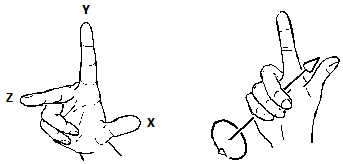
\includegraphics[width=0.5\linewidth]{img//Chapter_one/chaptOneManoDestra.png}
            \end{figure}
            \\
            Introduciamo l'operatore di rotazione $\hat{R}_{\underline{\varphi}}$ che effettua una rotazione attorno all'asse di rotazione specificata da $\underline{\varphi}$. Un mezzo è isotropo se risulta:
            \begin{equation}
                \hat{D}[\hat{R}_{\underline{\varphi}}(\underline{e}(\underline{r}, t))] = \hat{R}_{\underline{\varphi}}[\hat{D}(\underline{e}(\underline{r}, t))]  
            \end{equation}
            \\
            Assumendo ora che il mezzo sia anche non dispersivo nel tempo, dimostriamo che l'isotropia implica che la causa e l'effetto siano allineati, cioè che i vettori rappresentantin causa ed effetto siano fra loro proporzionali. \\
            Ipotizziamo che $\underline{e}(\underline{r},t)$ (causa) e $\underline{d}(\underline{r},t)$ (effetto) non siano tra loro allineati come in figura:
            \begin{figure}[h!]
                \centering
                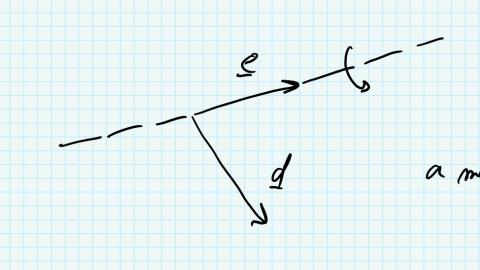
\includegraphics[width=0.5\linewidth]{img//Chapter_one/chaptOneIsotropia.png}
                \label{fig:isotropia}
                \caption{}
            \end{figure}
            Applicando una rotazione attorno all'asse corrispondente alla direzione di $\underline{e}(\underline{r},t)$, questo rimane invariato perché la rotazione di un vettore parallelo a quello di rotazione $\underline{\varphi}$ ritorna lo stesso vettore. Ciò però non si può dire per la causa, che invece varia. Ma poiché in principio abbiamo assunto che il mezzo sia isotropo, l'unica possibilità per la quale $\underline{d}(\underline{r},t)$ rimanga invariato per rotazione è che sia allineato a $\underline{e}(\underline{r},t)$. \\
            In generale non vale il contrario, cioè l'allineamento di $\underline{e}(\underline{r},t)$ e $\underline{d}(\underline{r},t)$ non implica l'isotropia. Per visualizzarlo, consideriamo un mezzo con la seguente relazione costitutiva:
            \begin{equation}
                \label{eqn:rel_cost_esempio}
                \underline{d}(\underline{r},t) = a(t) (\underline{e}(\underline{r},t) \cdot \underline{i}_{x})\underline{e}(\underline{r},t)
            \end{equation}
            Dalla (\ref{eqn:rel_cost_esempio}) traiamo le proprietà del mezzo: esso è non lineare (dipende dal prodotto per qualcosa che dipende da $\underline{e}(\underline{r},t)$), non dispersivo in $t$ ed in $\underline{r}$ (perché non c'è l'integrale in $\mathbb{R} ^{4}$), omogeneo nello spazio ed anisotropo\footnote{Per verificare l'anisotropia, valutare l'effetto della rotazione con due ingressi diversi, prima lungo l'asse $x$ e poi lungo $y$. Il secondo si annulla nel prodotto interno con $\underline{i}_{x}$, ottenendo in definitiva un risultato diverso da quello generato dal primo ingresso}.
            \\ \\
            Supponiamo ora di avere un mezzo lineare non dispersivo nel tempo e, come assunto già prima, nello spazio. Il risultato che stiamo per ottenere vale anche in assenza di non dispersività temporale. Vogliamo dimostrare la seguente catena di implicazioni:
            \begin{equation}
                \textrm{Isotropia} \implies \textrm{causa ed effetto allineati} \implies \underline{\underline{\varepsilon}} = \varepsilon \underline{\underline{I}} \implies \textrm{Isotropia}
            \end{equation}
            Cioè stiamo ambendo a dimostrare che per un mezzo lineare e non dispersivo nello spazio e nel tempo, se la causa e l'effetto sono allineati allora il mezzo è isotropo. La prima implicazione è stata dimostrata sopra. Per dimostrare la seconda, scriviamo la relazione costitutiva per un mezzo lineare e non dispersivo nello spazio e nel tempo:
            \begin{equation}
            \label{eqn:matricione1}
                \begin{pmatrix}
                    d_{x} \\
                    d_{y} \\
                    d_{z}
                \end{pmatrix} = 
                \begin{pmatrix}
                    \varepsilon_{xx} & \varepsilon_{xy} & \varepsilon_{xz} \\ 
                    \varepsilon_{yx} & \varepsilon_{yy} & \varepsilon_{yz} \\
                    \varepsilon_{zx} & \varepsilon_{zy} & \varepsilon_{zz} \\
                \end{pmatrix} \cdot 
                \begin{pmatrix}
                    e_{x} \\
                    e_{y} \\
                    e_{z}
                \end{pmatrix}
            \end{equation}
            dove l'elemento $\varepsilon_{ij}$ della matrice di permettività elettrica è la risposta in uscita lungo la direzione $i$ all'ingresso lungo la direzione $j$. Supponiamo di avere un ingresso lungo $x$:
            \begin{equation}
                \underline{e} = e_{0}\underline{i}_{x} = (e_{0} \quad 0 \quad 0\ )
            \end{equation}
            Sostituendo nella (\ref{eqn:matricione1}) otteniamo, sviluppando il prodotto matriciale a secondo membro:
            \begin{equation}
                \begin{cases}
                    d_{x} = \varepsilon_{xx} e_{0} \\
                    d_{y} = \varepsilon_{yx} e_{0} \\
                    d_{z} = \varepsilon_{zx} e_{0}
                \end{cases}
            \end{equation}
            Poiché causa ed effetto sono allineati, le risposte in uscita lungo $x$ dovute ad ingressi $y$ e $z$ devono essere nulle:
            \begin{equation}
                \varepsilon_{yx}=\varepsilon_{zx} = 0
            \end{equation}
            Iterando lo stesso procedimento per ingresso solo lungo $z$ e lungo $y$ si ottiene\footnote{Non è stato specificato in classe, ma ciò che ci permette di sommare i risultati ottenuti è la linearità, perché il generico ingresso di componenti $x,y,z$ può essere visto come combinazione lineare di ingressi lungo le singole direzioni}:
            \begin{equation}
            \label{eqn:matricione2}
                \underline{\underline{\varepsilon}} = \begin{pmatrix}
                    \varepsilon_{xx} & 0 & 0 \\
                    0 & \varepsilon_{yx} & 0 \\
                    0 & 0 & \varepsilon_{zx}
                \end{pmatrix}
            \end{equation}
            Affinché la permettività magnetica si possa scrivere come prodotto per la matrice identità $\underline{\underline{I}}$ ed una costante $\varepsilon$, dobbiamo dimostrare che i tre termini sulla diagonale siano tutti uguali. Consideriamo un ulteriore ingresso con componenti sul piano $xy$:
            \begin{equation}
                \underline{e} = e_{x}\underline{i}_{x}+e_{y}\underline{i}_{y}
            \end{equation}
            Sostituendo nella (\ref{eqn:matricione1}) e tenendo conto della (\ref{eqn:matricione2}) si ottiene:
            \begin{equation}
                \begin{cases}
                    d_{x} = \varepsilon_{xx}e_{x} \\
                    d_{y} = \varepsilon_{yy}e_{y}
                \end{cases}
            \end{equation}
            Dividendo membro a membro:
            \begin{equation}
            \label{eqn:matricione3}
                \frac{d_{y}}{d_{x}} = \frac{\varepsilon_{yy}}{\varepsilon_{xx}} \frac{\varepsilon_{y}}{\varepsilon_{x}}
            \end{equation}
            Disegnando i due vettori nel piano $xy$ ci si rende conto che (\ref{eqn:matricione3}) si può scrivere come:
            \begin{equation}
                \tan(\psi_{d}) = \frac{\varepsilon_{xx}}{\varepsilon_{yy}} \tan(\psi_{e})
            \end{equation}
            Ma se i due vettori sono allineati, allora hanno lo stesso angolo rispetto all'asse $x$ e di conseguenza:
            \begin{equation}
                \psi_{d} = \psi_{e} \implies \varepsilon_{xx} = \varepsilon_{yy}
            \end{equation}
            Reiterando il ragionamento per un ingresso nel piano $yz$ si arriva a:
            \begin{equation}
                \varepsilon_{xx} = \varepsilon_{yy} =\varepsilon_{zz} = \varepsilon
            \end{equation}
            \begin{figure}[h!]
                \centering
                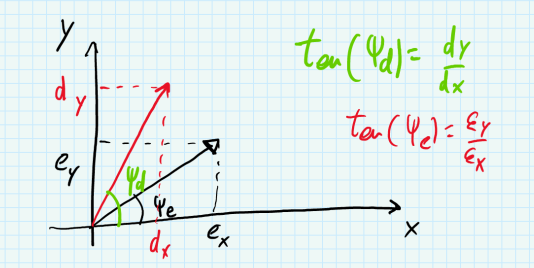
\includegraphics[width=0.5\linewidth]{img//Chapter_one/chaptOneMatricione.png}
            \end{figure}
            Resta da dimostrare l'ultima implicazione. A valle di ciò che abbiamo appena mostrato:
            \begin{equation}
                \underline{d}(\underline{r},t) = \varepsilon \underline{e}(\underline{r},t)
            \end{equation}
            Se applichiamo l'operatore di rotazione, che è un operatore lineare, la $\varepsilon$ che è una costante esce fuori dall'espressione e dunque si ottiene:
            \begin{equation}
                \hat{R}_{\underline{\varphi}}[\underline{d}(\underline{r},t)] = \varepsilon \hat{R}_{\underline{\varphi}}[\underline{e}(\underline{r},t)]
            \end{equation}
            ma causa ed effetto sono allineati e dunque la direzione di $\underline{d}$ ed $\underline{e}$ è la stessa, ragion per cui il mezzo è isotropo.

    \subsection{I mezzi normali e le relazioni nel dominio della frequenza}
        Un mezzo è detto \textbf{normale} se ha le seguenti proprietà:
        \begin{itemize}
            \item È lineare
            \item È non dispersivo nello spazio
            \item È stazionario
            \item È isotropo
        \end{itemize}
        A valle della definizione, le relazioni costitutive sono:
        \begin{equation}
            \begin{cases}
                \displaystyle\underline{d}(\underline{r},t) = \int_{\mathbb{R}}dt' g_{d}(\underline{r}, t-t')\underline{e}(\underline{r},t) \\
                \displaystyle\underline{b}(\underline{r},t) = \int_{\mathbb{R}}dt' g_{b}(\underline{r}, t-t')\underline{h}(\underline{r},t) \\
                \underline{j}(\underline{r}, t) = \sigma (\underline{r}) \cdot \underline{e}(\underline{r},t)
            \end{cases}
        \end{equation}
        Delle tre equazioni appena scritte, quella per la densità di corrente fa eccezione circa l'assunzione che il mezzo sia non dispersivo nel tempo, il quale ci permette di far saltare l'integrale e definire la conducibilità elettrica $\sigma(\underline{r})$. La proprietà di dispersivitò tuttavia rimane per $\underline{d}$ e $\underline{b}$. \\ \\
        Nel dominio di Fourier le stesse relazioni si scrivono come:
        \begin{equation}
            \begin{cases}
            
            \underline{D}(\underline{r},\omega) = \varepsilon (\underline{r}, \omega) \underline{E}(\underline{r}, \omega) \\
            \underline{B}(\underline{r} ,\omega) = \mu ( \underline{r}, \omega)  \underline{H}(\underline{r}, \omega) \\
            \underline{J}(\underline{r} ,\omega) = \sigma(\underline{r}) \underline{E}(\underline{r}, \omega)
            \end{cases}
        \end{equation}
        Analizziamo queste espressioni. Prima di tutto, sono prodotti di trasformate, perché nel tempo quegli integrali sono di convoluzione. In secundis, la permettività elettrica $\underline{\varepsilon}(\underline{r},t)$ e quella magnetica $\underline{\mu}(\underline{r},t)$ (che sono rispettivamente le trasformate di $g_{d}(\underline{r},t)$ e $g_{b}(\underline{r},t)$) dipendono dalla frequenza, cioè sono \textbf{dispersive in frequenza}. Un materiale è dispersivo in frequenza se il suo comportamento varia al variare della frequenza. Nel tempo, questo corrisponde alla dispersività nel tempo. Infatti, se il materiale è senza memoria (non dispersivo in $t$) l'integrale nel tempo salta e si ottiene:
        \begin{equation}
            \begin{cases}
            
            \underline{D}(\underline{r},\omega) = \varepsilon (\underline{r}) \underline{E}(\underline{r}, \omega) \\
            
            \underline{B}(\underline{r} ,\omega) = \mu ( \underline{r})\underline{H}(\underline{r}, \omega) \\
            
            \end{cases}
        \end{equation}
        ovvero la non dipendenza della funzione di Green ($\varepsilon$ e $\mu$ nel nostro caso) dalla frequenza. \\ \\
        Le equazioni di Maxwell, similmente, assumono questa forma qui:
        \begin{equation}
            \begin{cases}
            \nabla \times \underline{E} = - j \omega \underline{B} \\
            \nabla \times \underline{H} = j \omega \underline{D} + \underline{J} + \underline{J}_{0} \\
            \nabla \cdot \underline{D} = \rho + \rho_{0} \\
            \nabla \cdot \underline{B} = 0
            \end{cases}
        \end{equation}
    \section{Teoremi di unicità}
        Riprendiamo il discorso delle condizioni al contorno. Bisogna ricorrere ai teoremi di unicità, che offrono condizioni sufficienti (ma non necessarie!) a determinare univocamente la soluzione. I problemi di unicità sono classificati in quattro categorie:
        \begin{itemize}
            \item Problema interiore con soluzione nel tempo 
            \item Problema interiore con soluzione in frequenza
            
            \item Problema esteriore con soluzione nel tempo 
            \item Problema esteriore con soluzione in frequenza
        \end{itemize}
        Il problema è interiore quando si cerca la soluzione in un dominio $V$ limitato nello spazio, mentre è esteriore quando tale soluzione è cercata nel \textit{complemento} di un dominio limitato. Noi analizziamo i quattro casi considerando mezzi normali.
        \subsection{Problema tempo interiore}
        Iniziamo ad analizzare il caso "tempo-interiore" per cercare la soluzione nel dominio $V$. Assumendo la non dispersività temporale, assieme alle equazioni di Maxwell, che evito di riscrivere, bisogna scrivere le condizioni all'istante iniziale $t_{0}$:
        \begin{equation}
            \begin{cases}
                \underline{e}(\underline{r},t_{0}) = \underline{e}_{0}(\underline{r}) \\
                \underline{b}(\underline{r},t_{0}) = \underline{b}_{0}(\underline{r})
            \end{cases} \quad \forall \underline{r} \in V
        \end{equation}
        Vanno poi aggiunte le equazioni costitutive per un mezzo normale non dispersivo in $t$:
        \begin{equation}
        \begin{cases}
            \underline{d}(\underline{r},t) = \underline{\varepsilon}(\underline{r}) \underline{e}(\underline{r},t) \\
            \underline{b}(\underline{r},t) = \mu (\underline{r}) \underline{h}(\underline{r},t) \\
            \underline{j}(\underline{r},t) = \sigma ( \underline{r}) \underline{e}(\underline{r},t)
        \end{cases}
        \end{equation}
        Ultime ma non meno importanti le condizioni al raccordo:
        \begin{equation}
            \underline{i}_{n} \times \underline{e}(\underline{r}, t) = \underline{e}_{tg}(\underline{r},t) \qquad \underline{r} \in \partial V, \ \ t \geq t_{0}
        \end{equation}
        Il teorema di unicità per il problema tempo interiore afferma che date queste informazioni, cioè equazioni di Maxwell, raccordo, costitutive e condizioni iniziali, la soluzione se esiste è unica. Il teorema di unicità è una condizione sufficiente ma non necessaria. \\
        Per dimostrare il teorema, introduciamo il \textbf{vettore di Poynting}, la cui trattazione è posticipata ai capitoli successivi:
        \begin{equation}
            \underline{s} = \underline{e} \times \underline{h}
        \end{equation}
        Calcoliamo allora la divergenza del vettore di Poynting:
        \begin{equation}
            \nabla \cdot \underline{s}  = \nabla \cdot (\underline{e} \times \underline{h}) = \nabla \times \underline{e} \cdot \underline{h}-\underline{e} \nabla \times \underline{h}
        \end{equation}
        dove nell'ultimo passaggio abbiamo utilizzato un'identità vettoriale notevole.\footnote{$\nabla \cdot (\underline{a} \times \underline{b}) = \nabla \times \underline{a} \cdot \underline{b} - \underline{a} \cdot \nabla \times \underline{b}$}
        Sostituendo le espressioni dei rotori di $\underline{e}$ ed $\underline{h}$ dateci dalle equazioni di Maxwell:
        \begin{equation}
            \nabla \cdot \underline{s} = (-\frac{\partial}{\partial t} \underline{b})\cdot \underline{h}-\underline{e} \cdot (\frac{\partial}{\partial t}\underline{d}+\underline{j}+\underline{j}_{0})
        \end{equation}
        Riordinando l'equazione si ottiene \textbf{l'identità di Poynting in forma locale}:
        \begin{equation}
            \nabla \cdot \underline{s} +\underline{h} \cdot \frac{\partial}{\partial t} \underline{b}+\underline{e} \cdot \frac{\partial}{\partial t}\underline{d}+\underline{e} \cdot \underline{j}= \underline{e} \cdot \underline{j}_{0}
        \end{equation}
        Si ottiene l'identità di Poynting in forma integrale semplicemente integrando su $V$ e applicando il teorema di Gauss per la divergenza di $\underline{s}$ si ottiene:
        \begin{equation}
            \oiint_{\partial V} \underline{s} \cdot \underline{i}_{n} dS + \iiint_{V} ( \underline{h} \cdot \frac{\partial}{\partial t} \underline{b}+\underline{e}\cdot \frac{\partial}{\partial t} \underline{d})dV + \iiint_{V} \underline{e} \cdot \underline{j}dV = - \iiint_{V} \underline{e} \cdot \underline{j}_{0} dV
        \end{equation}
        Finora non abbiamo sfruttato le ipotesi nel mezzo, ma non è mai tardi per cambiare idea.
        Sostituiamo le relazioni costitutive per un mezzo normale non dispersivo nel tempo:
        \begin{equation}
            \underline{b} = \mu \cdot \underline{h} \quad \underline{d} = \varepsilon \cdot \underline{e} \quad \underline{j} = \sigma \cdot \underline{e}
        \end{equation}
        \begin{equation}
            \implies \nabla \cdot \underline{s} + \underline{h} \frac{\partial}{\partial t}(\mu \cdot \underline{b})+\underline{e} \cdot \frac{\partial}{\partial t}(\varepsilon \cdot \underline{e})+(\sigma \cdot \underline{e}) \cdot \underline{e} = -\underline{e} \cdot \underline{j}_{0}
        \end{equation}
        Invocando la stazionarietà, $\mu$, $\varepsilon$ e $\sigma$ escono fuori dalle derivate. Notiamo che possiamo scrivere:
        \begin{equation}
           \mu \cdot \underline{h} \cdot \frac{\partial}{\partial t} (\underline{h}) = \frac{\mu}{2} \cdot \frac{\partial}{\partial t} (\underline{h}^{2}) = \frac{\mu}{2} \cdot \frac{\partial}{\partial t}|h|^{2}
        \end{equation}
        \begin{equation}
            \varepsilon \cdot \underline{e} \cdot \frac{\partial}{\partial t} \underline{e} = \varepsilon \frac{\partial}{\partial t} |\underline{e}|^{2}
        \end{equation}
        \begin{equation}
            \sigma \underline{e} \cdot \underline{e} = \sigma |e|^{2}
        \end{equation}
        potendo scrivere, in definitiva:
        \begin{equation}
            \nabla \cdot \underline{s} + \frac{\partial}{\partial t}(\frac{\mu}{2} |\underline{h}|^{2}+\frac{\varepsilon}{2}|\underline{e}|^{2}) = - \underline{e} \cdot \underline{j}_{0}
        \end{equation}
        ovvero l'identità di Poynting in forma locale per mezzi normali non dispersivi.
        Per la forma integrale, ammesso che $V$ non vari nel tempo:
        \begin{equation}
            \oiint_{\partial V} \underline{s} \cdot \underline{i}_{n} dS + \frac{d}{dt}\iiint_{V} \frac{\mu}{2} |\underline{h}|^{2}+\frac{\varepsilon}{2}|\underline{e}|^{2}dV + \iiint_{V} \sigma |\underline{e}|^{2} dV = - \iiint_{V} \underline{e}\cdot \underline{j}_{0}dV
        \end{equation}
        Importante notare il simbolo di derivata totale rispetto al tempo al posto di quella parziale, in quanto la dipendenza spaziale di $\underline{e}$ ed $\underline{h}$ viene persa a causa dell'integrazione in $V$. \\ \\
        Ora possiamo finalmente dimostrare il teorema di unicità per il caso tempo-interno. 
        Supponiamo che la soluzione esista e che per assurdo sia non unica, dunque ce ne sono almeno due, per esempio $(\underline{e}_{1}, \underline{h}_{1})$ e $(\underline{e}_{2}, \underline{h}_{2})$. \\
        Sostituiamo le equazioni costitutive all'interno di quelle di Maxwell, ottenendo un sistema con sole incognite $\underline{e}$ ed $\underline{h}$.
        \begin{equation}
            \begin{cases}
            \nabla \times \underline{e} = - \displaystyle \mu \cdot \frac{\partial}{\partial t} \underline{h} \\
            \nabla \times \underline{h} = \displaystyle \varepsilon \cdot \frac{\partial}{\partial t} \\
            \nabla \cdot \underline{d} = \rho + \rho_{0} \\
            \nabla \cdot (\mu \underline{h}) =0
            \end{cases}
        \end{equation}
        Si tenga conto che $\underline{j}$ è ricavabile conoscendo $\underline{e}$ ed $\underline{h}$ in virtù dell'equazione di continuità\footnote{Che ricordiamo essere $\nabla \cdot j = - \displaystyle \frac{\partial}{\partial t}\rho $}.\\
        Definiamo i vettori differenza $\underline{e}_{d}$ ed $\underline{h}_{d}$:
        \begin{equation}
            \begin{cases}
                \underline{e}_{d} = \underline{e}_{1}-\underline{e}_{2} \\
                \underline{h}_{d} = \underline{h}_{1} - \underline{h}_{2}
            \end{cases}
        \end{equation}
        Vogliamo verificare che siano anch'essi campi elettromagnetici. Se $\underline{e}_{1}$ ed $\underline{e}_{2}$, così come $\underline{h}_{1}$ ed $\underline{h}_{2}$, sono soluzioni, allora devono soddisfare le equazioni di Maxwell. Se sostituiamo nella prima, si ottiene:
        \begin{equation}
        \begin{cases}
            \nabla \times \underline{e}_{1} = -  \displaystyle \mu \frac{\partial}{\partial t} \underline{h}_{1} \\
            \nabla \times \underline{e}_{2} = - \mu \frac{\partial}{\partial t} \underline{h}_{2}
        \end{cases} \implies \nabla \times (\underline{e}_{2}-\underline{e}_{1}) = - \mu \frac{\partial}{\partial t}(\underline{h}_{2}-\underline{h}_{1})
        \end{equation}
        ovvero:
        \begin{equation}
            \nabla \times \underline{e}_{d} = - \mu \frac{\partial}{\partial t} \underline{h}_{d}
        \end{equation}
        La prima è soddisfatta. Reiterando il ragionamento, anche la seconda è soddisfatta \textbf{ma con termine noto nullo}:
        \begin{equation}
        \begin{cases}
            \nabla \times \underline{h}_{1} = \displaystyle \varepsilon \cdot \frac{\partial}{\partial t} \underline{e}_{1} + \sigma \underline{e}_{1} + \underline{j}_{0} \\
            
            \nabla \times \underline{h}_{2} = \displaystyle \varepsilon \cdot \frac{\partial}{\partial t} \underline{e}_{2} + \sigma \underline{e}_{2} + \underline{j}_{0}
        \end{cases} \implies \nabla  \times \underline{h}_{d} = \varepsilon \frac{\partial}{\partial t} \underline{e}_{d} + \sigma \underline{e}_{d}
        \end{equation}
        Similmente, per la terza si ricava:
        \begin{equation}
            \varepsilon \nabla \cdot \underline{e}_{d} = \rho
        \end{equation}
        mentre della quarta è inutile discutere. \\
        Otteniamo in definitiva un sistema di equazioni omogenee:
        \begin{equation}
        \begin{cases}
            \nabla \times \underline{e}_{d} = - \displaystyle \mu \frac{\partial}{\partial t} \underline{h}_{d} \\
            \nabla \times \underline{h}_{d} = \displaystyle \varepsilon \frac{\partial}{\partial t} \underline{e}_{d}+\sigma \cdot \underline{e}_{d} \\
            \nabla \cdot (\varepsilon \underline{e}_{d}) = \rho \\
            \nabla \cdot (\mu \underline{h}_{d} )= 0
        \end{cases}
        \end{equation}
        Poiché le due soluzioni che abbiamo supposto valide prima hanno le stesse condizioni iniziali ed al contorno, quelle relative ai vettori differenza sono nulle:
        \begin{equation}
            \begin{cases}
                \underline{e}_{d} (\underline{r},t_{0}) = 0 \\
                \underline{h}_{d} (\underline{r},t_{0})=0
            \end{cases}
        \end{equation}
        \begin{equation}
            \underline{i}_{n} \times \underline{e}_{d}(\underline{r},t) = 0
        \end{equation}
        Segue che i vettori differenza sono campi elettromagnetici. Applicando Poynting per mezzi normali non dispersivi nel tempo:
        \begin{equation}
            \oiint_{\partial V} \underline{s}_{d} \cdot \underline{i}_{n} dS + \frac{d}{dt} \iiint_{V} (\frac{\mu}{2} |\underline{h}_{d}|^{2}+\frac{\varepsilon}{2}|\underline{e}|^{2})dV + \iiint_{V} \sigma |\underline{e}_{d}|^{2}dV = - \iiint_{V} \underline{e} \cdot \underline{j}_{0}dV
        \end{equation}
        Il termine:
        \begin{equation}
            \iiint_{V} \underline{e} \cdot \underline{j}_{0}dV
        \end{equation}
        va a zero perché per i vettori differenza i termini noti sono nulli. Similmente, esprimendo $\underline{s}_{d}$:
        \begin{equation}
            \underline{s}_{d} = \underline{e}_{d} \times \underline{h}_{d} \cdot \underline{i}_{n} = \underline{i}_{n} \times \underline{e}_{d} \cdot \underline{h}_{d} = 0 \cdot \underline{h}_{d} = 0
        \end{equation}
        avendo sfruttato le condizioni al contorno per i vettori differenza.
        Supponendo che:
        \begin{equation}
            \begin{cases}
                \mu > 0 \\
                \varepsilon > 0 \\
                \sigma \geq 0
            \end{cases}
        \end{equation}
        e definendo:
        \begin{equation}
            P_{j}(t) = \iiint_{V} \sigma |\underline{e}|^{2}dV \qquad W(t) = \iiint_{V} (\frac{\mu}{2}|\underline{h}|^{2}+\frac{\varepsilon}{2}|\underline{e}|^{2})dV
        \end{equation}
        si ricava dall'identità di Poynting:
        \begin{equation}
            \frac{d}{dt}W(t) = - P_{J}(t)
        \end{equation}
        In virtù delle ipotesi su $\sigma, \varepsilon$ e $\mu$, si ottiene $P_{J}(t) \geq 0 \ \ \forall t$ e dunque la derivata di $W(t)$ è non positiva. Ciò significa che:
        \begin{equation}
            t \geq t' \implies W(t) \geq W(t')
        \end{equation}
        Per cui fissato l'istante iniziale $t_{0}$:
        \begin{equation}
            W(t_{0}) \geq W(t) \quad \forall t \geq t_{0}
        \end{equation}
        Tuttavia, per come $W(t)$ è definita, sotto le ipotesi fatte per $\sigma, \varepsilon$ e $\mu$, è una funzione semidefinita positiva, cioè $W(t) \geq 0$. Dunque:
        \begin{equation}
            0 \leq W(t) \leq 0 \implies W(t) = \iiint_{V} \frac{\mu}{2}|\underline{h}_{d}|^{2}+\frac{\varepsilon}{2}|\underline{e}_{d}|^{2}dV = 0
        \end{equation}
        Si può passare dall'integrale all'integrando nullo perché l'integrando è semidefinito nel segno, in quanto ci sono tutte quantità non negative. L'unico modo per il quale l'integrando si annulla, poiché $\mu >0$ e $\varepsilon>0$ è:
        \begin{equation}
            |\underline{h}_{d}|^{2} = |\underline{e}_{d}|^{2} = 0 \implies \underline{h_{1}}=\underline{h}_{2} \qquad \underline{e}_{1} = \underline{e}_{2}
        \end{equation}
        QED. \\ \\
        Se avessimo assegnato come condizione al contorno:
        \begin{equation}
            \underline{i}_{n} \times \underline{h} = \underline{h}_{tg}
        \end{equation}
        bastava fare una permutazione circolare diversa per l'espressione di $\underline{s}_{d}$ e trovare lo stesso risultato. \textbf{Non} si possono dare entambe le condizioni perché se do una identifico univocamente anche l'altra. In altre parole, se ho sia la condizione di contorno per il campo elettrico che per quello magnetico il sistema di equazioni è incompatibile e non ammette soluzione.
        \newpage
        \subsection{Problema tempo-esteriore}
            Per il problema tempo esteriore, dobbiamo considerare il complemento di un dominio limitato, per esempio:
            \begin{figure}[h!]
                \centering
                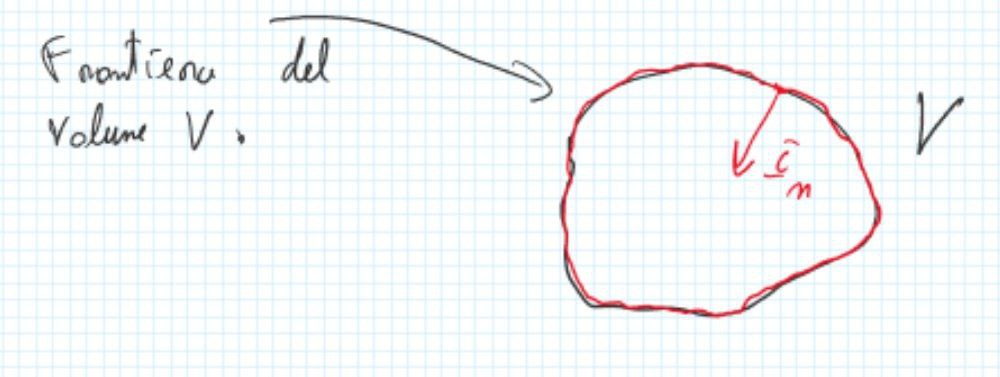
\includegraphics[width=0.5\linewidth]{img//Chapter_one/Chapt1img8.png}
            \end{figure}
        Se consideriamo una superficie sferica sufficientemente grande che racchiude una buona porzione di spazio attorno a $V$, potremmo pensare di risolvere il problema esteriore come un problema interiore nella regione di spazio intermedio fra $V$ e la frontiera della superficie sferica. Il problema è che non si conoscono le condizioni del campo sulla frontiera di tale sfera. \\
        Ipotizziamo allora di stare nelle condizioni per cui il campo è zero definitivamente in un intorno dell'infinito, cioè esiste sempre un intorno dell'infinito per il quale il campo è nullo. Questo ha senso se si considera la causalità forte, che richieda lo scorrere di un intervallo di tempo non nullo affinché gli effetti delle sorgenti si propaghino nello spazio. Tutto questo ragionamento crolla per la soluzione a regime, dove di tempo ne è passato idealmente infinito rispetto all'accensione delle sorgenti di campo, abbastanza per raggiungere ogni punto dello spazio con gli effetti. \\ 
        In definitiva, la risoluzione del problema tempo-esteriore deriva direttamente da quella del caso tempo-interiore, nel caso in cui non sia interessati alla soluzione a regime.

    \subsection{Problema omega-interiore}
        Il teorema di unicità omega-interiore richiede che vengano fornite le equazioni di Maxwell:
        \begin{equation}
        \begin{cases}
            \nabla \times \underline{E} = -j \omega \underline{B} \\
            \nabla \times \underline{D} = j \omega \underline{D}+\underline{J}+\underline{J}_{0} \\
            \nabla \cdot \underline{D} = \rho \\
            \nabla \cdot \underline{B} = 0
        \end{cases}
        \end{equation}
        le relazioni costitutive - nel nostro caso per i mezzi normali:
        \begin{equation}
            \begin{cases}
                \underline{D}(\underline{r},\omega) = \varepsilon(\underline{r})  \underline{E}(\underline{r},\omega) \\
                \underline{B}(\underline{r},\omega) = \mu(\underline{r})\underline{H}(\underline{r},\omega) \\
                \underline{J}(\underline{r},\omega) = \sigma(\underline{r})\underline{E}(\underline{r},\omega)
            \end{cases}
        \end{equation}
        e infine le relazioni al contorno:
        \begin{equation}
            \underline{i}_{n} \times \underline{E}|_{\partial V} = \underline{E}_{tg}
        \end{equation}
        dove $\underline{i}_{n} \times E|_{\partial V}$ è la componente tangente\footnote{ruotata di $\pi/2$ ndr} del campo elettrico calcolata sulla frontiera di $V$. \\
        Delle condizioni iniziali non ce ne facciamo niente perché 1) stiamo cercando la soluzione in regime sinusoidale e 2)in frequenza per includerle si dovrebbe fare un casino matematico.
        Il teorema afferma che date queste informazioni la soluzione se esiste è unica in \textbf{a meno di condizioni risonanti}. \\ \\
        Procediamo in modo analogo a quanto fatto per il tempo interiore introducendo il vettore di Poynting nel dominio della frequenza:
        \begin{equation}
            \underline{S}=\frac{1}{2}\underline{E} \times \underline{H}^{*}
        \end{equation}
        Calcoliamone a divergenza:
        \begin{equation}
            \nabla \cdot \underline{S} = \nabla \cdot (\frac{1}{2}\underline{E} \times \underline{H}^{*}) = \frac{1}{2}[\nabla \times \underline{E} \cdot \underline{H}^{*}- \underline{E} \cdot \nabla \times \underline{H}^{*}]
        \end{equation}
        Sostituiamo le equazioni di Maxwell per levare $\underline{D}$ e $\underline{B}$:
        \begin{equation}
            \nabla \cdot \underline{S} = j \frac{\omega}{2}(\mu \underline{H}) \cdot \underline{H}^{*}-j \frac{\omega}{2}(\varepsilon \underline{E})^{*}\cdot \underline{E} + \frac{1}{2}\underline{E} \cdot (\sigma \underline{E})^{*} 0 \frac{1}{2}\underline{E} \cdot \underline{J}_{0} 
        \end{equation}
        A valle che fatto che $\sigma$ non dipende dal tempo, la sua trasformata in $\omega$ è un numero reale, mentre $\mu$ e $\varepsilon$ sono complessi:
        \begin{equation}
            \nabla \cdot \underline{S} = j \frac{\omega}{2}\mu\cdot  (\underline{H} \cdot \underline{H}^{*})-j \frac{\omega}{2}\varepsilon^{*} (\underline{E}^{*}\cdot \underline{E}) + \frac{1}{2}\sigma^{*}(\underline{E} \cdot  \underline{E})^{*} = -\frac{1}{2} \underline{E}\cdot \underline{J}_{0}
        \end{equation}
        Riconosciamo nell'espressione i moduli di $\underline{H} $ ed $ \underline{E}$\footnote{Vedi appendice A per note sulla norma dei vettori complessi}, potendo dunque scrivere:
        \begin{equation}
        \label{eqn:rel_stronza}
            \nabla \cdot \underline{S} +j \omega \frac{\mu}{2}|\underline{H}|^{2}-j \frac{\omega}{2}\varepsilon^{*}|\underline{E}|^{2}+\frac{\sigma}{2}|\underline{E}|^{2}=-\frac{1}{2}\underline{E} \cdot \underline{J}_{0}
        \end{equation} \\
        Scomponiamo la (\ref{eqn:rel_stronza}) come coppia di equazioni, una alla parte reale e una alla parte immaginaria di $\nabla \cdot \underline{S}$. Posto:
        \begin{equation}
            \underline{S}=\underline{S}_{R}+j\underline{S}_{I} \qquad \varepsilon=\varepsilon'-j\varepsilon'' \qquad \mu = \mu'-j\mu''
        \end{equation}
        dove $\varepsilon''$ e $\mu''$ sono gli opposti delle parti immaginarie di $\varepsilon$ e $\mu$, definite per facilità di calcolo, si può scrivere per quella reale:
        \begin{equation}
            \nabla \cdot \underline{S}_{R} = \Re[j \frac{\omega}{2}\mu |H|^{2}]-\Re[j \frac{\omega}{2}\varepsilon^{*}|E^{2}|]+\Re[\frac{\sigma}{2}|E|^{2}]-\frac{1}{2}\Re[\underline{E}\cdot \underline{J}_{0}]
        \end{equation}
        \begin{equation}
            \implies 
            \nabla \cdot \underline{S}_{R} = \frac{\omega}{2}|H|^{2}\Re[j \mu]-|E^{2}|\frac{\omega}{2}\Re[j \varepsilon^{*}]+\frac{\sigma}{2}|E|^{2}-\frac{1}{2}\Re[\underline{E}\cdot \underline{J}_{0}]
        \end{equation}
        Ora poiché $z \in \mathbb{C} \implies \Re[j z]=-\Im[z]$\footnote{$\Re[jz] = \Re[jz_{R}-z_{I}] = -z_{I}$}, si ottiene:
        \begin{equation}
            \Re[j\mu] = \mu '' \qquad \Re[j \varepsilon^{*}] = - \varepsilon''
        \end{equation}
        Ottenendo:
        \begin{equation}
            \nabla \cdot \underline{S}_{R}+\frac{\omega}{2}|\underline{H}|^{2}\mu''+\frac{\omega}{2}|\underline{E}|^{2}\varepsilon''+\frac{\sigma}{2}|\underline{E}|^{2}=-\Re[\frac{1}{2}\underline{E}\cdot \underline{J}_{0}]
        \end{equation}
        Mentre per la parte immaginaria\footnote{dove abbiamo rimosso a priori $\sigma |\underline{E}|^{2}$ che è totalmente reale}:
        \begin{equation}
            \nabla \underline{S}_{I} +\frac{\omega}{2}|\underline{H}|^{2} \textrm{Im}[j \mu]-\frac{\omega}{2}|\underline{E}|^{2}\textrm{Im}[j \varepsilon^{*}] = - \textrm{Im}[\frac{1}{2}\underline{E}\cdot \underline{J}_{0}]
        \end{equation}
        Ottenendo, in virtù di $\textrm{Im}[jz]=\Re[z]$:
        \begin{equation}
            \nabla \cdot \underline{S}_{I}+\frac{\omega}{2}|\underline{H}|^{2}\mu'-\frac{\omega}{2}|\underline{E}|^{2}\varepsilon'=-\textrm{Im}[\frac{1}{2}\underline{E}\cdot \underline{J}_{0}]
        \end{equation}
        Mettendo a sistema, ricaviamo l'identità di Poynting in forma locale come equazioni alla parte reale e immaginaria:
        \begin{equation}
        \begin{cases}
            \nabla \cdot \underline{S}_{R}+\frac{\omega}{2}|\underline{H}|^{2}\mu''+\frac{\omega}{2}|\underline{E}|^{2}\varepsilon''+\frac{\sigma}{2}|\underline{E}|^{2}=-\Re[\frac{1}{2}\underline{E}\cdot \underline{J}_{0}] \\
             \nabla \cdot \underline{S}_{I}+\frac{\omega}{2}|\underline{H}|^{2}\mu'-\frac{\omega}{2}|\underline{E}|^{2}\varepsilon'=-\textrm{Im}[\frac{1}{2}\underline{E}\cdot \underline{J}_{0}]
        \end{cases}
        \end{equation}
        Per passare alla forma integrale, si raccoglie un $2\omega$ alla parte immaginaria per convenzione e si integra in $V$, applicando Gauss per il flusso di $\underline{S}$:
        \begin{equation}
            \begin{cases}
             \displaystyle \oiint_{\partial V}  \underline{S}_{R} \cdot \underline{i}_{n}dV+\iiint_{V} (\frac{\omega}{2}|\underline{H}|^{2}\mu''+\frac{\omega}{2}|\underline{E}|^{2}\varepsilon'')dV+\iiint_{V}\frac{\sigma}{2}|\underline{E}|^{2}dV=-\Re[\iiint_{V}\frac{1}{2}\underline{E}\cdot \underline{J}_{0} dV] \\ \\
             \displaystyle \oiint_{\partial V}  \underline{S}_{I} \cdot \underline{i}_{n}+ 2 \omega\iiint_{V} \frac{\omega}{4}|\underline{H}|^{2}\mu'dV-2 \omega\iiint_{V}\frac{\omega}{4}|\underline{E}|^{2}\varepsilon'dV=-\textrm{Im}[\iiint_{V}\frac{1}{2}\underline{E}\cdot \underline{J}_{0}dV]
        \end{cases}
        \end{equation}
         \\ \\
         Ricavata l'identità di Poynting in frequenza, possiamo dimostrare il teorema. In modo analogo al caso tempo-interiore, ipotizziamo per assurdo che ci siano almeno due soluzioni $(\underline{E}_{1}, \underline{H}_{1})$ e $(\underline{E}_{2}, \underline{H}_{2})$. Diamo per assodato che i vettori differenza:
         \begin{equation}
             \underline{E}_{d} = \underline{E}_{1}-\underline{E}_{2} \qquad \underline{H}_{d}=\underline{H}_{1}-\underline{H}_{2}
         \end{equation}
         soddisfino le equazioni di Maxwell con condizioni al raccordo e termini noti nulli, come abbiamo fatto vedere nel caso temporale sostituendo le soluzioni nelle relazioni e sottraendo membro a membro:
         \begin{equation}
             \rho_{0, d} = 0 \qquad J_{0, d} = \underline{0} \qquad  \underline{i}_{n} \times \underline{E}_{d}|_{\partial V}  = \underline{0}
         \end{equation}
         Applichiamo l'identità di Poynting tenendo conto di quanto appena scritto per i vettori differenza. Come nel caso tempo-interno, il flusso del vettore di Poynting risulta nullo in virtù della nullità della componente tangente del campo elettrico $E_{tg, d}$
         \begin{equation}
             \underline{S}_{d} \cdot \underline{i}_{n}=\frac{1}{2} \underline{E}_{d} \times \underline{H}_{d} \cdot \underline{i}_{n} =\frac{1}{2} \underline{i}_{n} \times \underline{E}_{d} \cdot \underline{H}_{d} = \frac{1}{2} \cdot 0 \cdot \underline{H}_{d} = 0
         \end{equation}
         In modo analogo, i termini a secondo membro dell'identità di Poynting, sia per la parte reale che immaginaria, sono nulli per la nullità di $\underline{J}_{0, d}$. Scriviamo in definitiva:
         \begin{equation}
             \begin{cases}
                 \displaystyle \iiint_{V}\frac{\mu''}{2}|\underline{H}|^{2}+\frac{\varepsilon''}{2}|\underline{E}|dV+\iiint_{V} \frac{\sigma}{2}|\underline{E}_{d}|^{2}dV = 0 \\ \\

                \displaystyle 2 \omega [\iiint_{V} \frac{\mu''}{4}|\underline{H}|^{2}dV - \iiint_{V} \frac{\varepsilon'}{4}|\underline{E}|^{2}dV]= 0
             \end{cases}
         \end{equation}
Ipotizziamo:
\begin{equation}
    \begin{cases}
        \omega \varepsilon''>0 \\
        \omega \mu'' > 0 \\
        \sigma \geq 0
    \end{cases} \qquad \qquad \omega \neq 0
\end{equation}
Le trasformate delle funzioni di Green $\mu, \varepsilon$ e $\sigma$ sono trasformate di funzioni reali, dunque il loro spettro è hermitiano. Per simmetria hermitiana, la parte immaginaria è una funzione dispari. Poiché la funzione $y=\omega$ è dispari\footnote{È la bisettrice del primo quadrante} allora le $\omega \varepsilon''$ ed $\omega \mu''$ sono funzioni pari, dunque sono positive per omega positive, zero per omega nulle e negative altrimenti. Consideriamo allora l'equazione per la parte reale:
\begin{equation}
    \iiint_{V}\frac{\mu''}{2}|\underline{H}|^{2}+\frac{\varepsilon''}{2}|\underline{E}|dV+\iiint_{V} \frac{\sigma}{2}|\underline{E}_{d}|^{2}dV = 0
\end{equation}
L'integrale  è nullo perché semidefinito nel segno. Si può passare all'integrando nullo perché le quantità sotto segno di integrale sono tutte non negative, per cui vale la legge di annullamento del prodotto. L'unico modo per cui l'espressione è nulla è che:
\begin{equation}
    |\underline{H}_{d}|=|\underline{E}_{d}|=0
\end{equation}
da cui la tesi.
Ipotizziamo ora che $\omega \mu'' = 0, \sigma =0, \omega \varepsilon''>0$. In tal caso sostituendo nella relazione per la parte reale risulta $|\underline{E_{d}}|=0$. Sostituendo poi nella prima equazione di Maxwell:
\begin{equation}
    \nabla \times \underline{E}_{d} = 0 = -j \omega \mu \underline{H}_{d} \implies \underline{H}_{d}=0
\end{equation}
da cui di nuovo l'unicità della soluzione. Possiamo reiterare lo stesso ragionamento ponendo una variable maggiore di zero e le altre due nulle. Cosa accade se sono tutte e tre nulle? Che l'equazione parte reale si annulla, non potendone ricavare alcuna informazione, mentre quella parte immaginaria diventa:
\begin{equation}
    \iiint_{V} \frac{\mu'}{4}|\underline{H}_{d}|^{2}dV = \iiint_{V} \frac{\varepsilon'}{4}|\underline{E}_{d}|^{2}dV
\end{equation}
In tal caso la soluzione non è unica e l'unico costringente che si ha è l'uguaglianza integrale che abbiamo appena scritto: questo è il caso delle \textbf{soluzioni risonanti}. Fisicamente parlando, la parte reale è costituta dai termini del problema elettromagnetico responsabili delle perdite di energia. Nel caso di soluzione risonante, il circuito oscilla in modo indefinito in assenza sia di forzamenti interni, dovuti a $\rho_{0}$ e $\underline{J}_{0}$, che esterni, dovuti alle condizioni al contorno che rappresentano l'influenza dei campi elettromagnetici esterni.

\subsection{Problema omega-esteriore}
    Nel caso temporale, abbiamo considerato soluzioni non a regime, per avvalerci del fatto che esiste sempre un intorno di infinito per il quale il campo è definitivamente nullo. Per le soluzioni in frequenza, che nel nostro caso sono sempre a regime sinusoidale, non possiamo più fare questa cosa senza ipotizzare che valga la seguente:
    \begin{equation}
        \lim_{\underline{r} \to \infty} \underline{r}(\underline{E}-\zeta \underline{H} \times \underline{i}_{r}) = 0
    \end{equation}
    detta \textbf{condizione di radiazione all'infinito} oppure di \textbf{Silver-M{\"u}ller}. La tesi, che non dimostriamo, afferma che sotto tale ipotesi la soluzione se esiste è unica e non possono esserci soluzioni risonanti. Intuitivamente\footnote{l'espressione che segue è da considerarsi una chiacchiera da bar, non pretende di essere formale} questa cosa è associata al fatto che la radiazione propagandosi all'infinito senza tornare indietro si porti appresso dell'energia, la quale viene sottratta al sistema fino ad esaurirsi.
\section{Il teorema di Poynting}
    \subsection{Energia legata al campo elettromagnetico}
        Il primo principio della termodinamica afferma che la variazione dell'energia interna $U$
        di un sistema fisico varia in accordo agli scambi energetici del sistema con l'esterno.
        In altre parole, la variazione di energia interna è pari alla variazione di calore $\delta Q$ e lavoro $\delta L$:
        \begin{equation}
            \label{eqn:primo_principio_termodinamica}
            d U = \delta Q+\delta L
        \end{equation}
    \subsection{Teorema di Poynting nel dominio del tempo}
        Fatta l'ipotesi di mezzo normale non dispersivo nel tempo, vale la già discussa identità di Poynting in forma integrale:
        \begin{equation}
            \label{eqn:Poynting_integrale_tempo}
            \oiint_{\partial V} \underline{s} \cdot \underline{i}_{n}dS+\frac{d}{dt}\iiint_{V}(\frac{\mu}{2}|\underline{h}|^{2}+\frac{\varepsilon}{2}|\underline{e}|^{2})dV +
            \iiint_{V}\sigma |\underline{e}|^{2}dV = - \iiint_{V} \underline{e}\cdot \underline{j}_{0}dV
        \end{equation}
        L'obiettivo di questa sottosezione è ricostruire l'identità di Poynting in modo analogo alla (\ref{eqn:primo_principio_termodinamica}), per associare ad ogni pezzo della
        (\ref{eqn:Poynting_integrale_tempo}) il suo significato fisico. \\
        Partiamo dall'espressione della forza di Lorentz esercitata su di una carica $q$:
        \begin{equation}
            \underline{F}= q \underline{e}+\rho \underline{r} \times \underline{b}
        \end{equation}
        La forza di Lorentz è un approccio macroscopico al problema della forza esercitata su di una carica immersa in un campo elettromagnetico, perché compare la densità di carica
        elettrica $\rho$, dunque le cariche vengono immaginate come un continuo nello spazio. Consideriamo allora un volumetto $\Delta V$ con all'interno carica $\Delta q$.
        Calcolando la forza di Lorentz esercitata su tale volumetto di carica:
        \begin{equation}
            \Delta \underline{F} = \Delta q\underline{e}+\Delta \rho \underline{r}\times \underline{b}
        \end{equation}
        Passiamo alla densità di forza, (misurata in $N/m^{3}$) dividendo per $\Delta V$ e facendo il limite per $\Delta V \to 0$:
        \begin{equation}
            \label{eqn:densitaForza}
            \lim_{\Delta V \to \infty} \frac{\Delta \underline{F}}{\Delta V} = \underline{f}(\underline{r},t) = \rho(\underline{r},t)\underline{e}(\underline{r},t)+\rho(\underline{r},t)\underline{v}\times \underline{b}(\underline{r},t)
        \end{equation}
        Il primo addendo della (\ref{eqn:densitaForza}) deriva direttamente della definizione di densità di carica, semplicemente il limite del rapporto $\Delta q/\Delta V$.
        Per capire che significato abbia il secondo addendo, consideriamo una superficie con piana orientata lungo l'asse $x$, cioè con $\underline{i}_{n} = \underline{i}_{x}$:
        \begin{figure}[h!]
            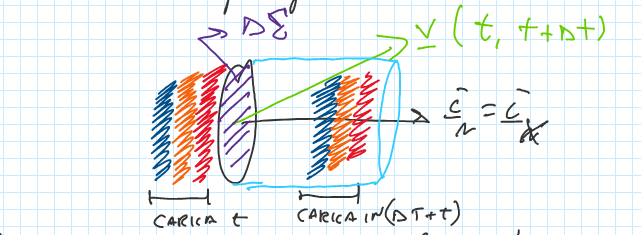
\includegraphics[width=0.6\linewidth]{img/Chapter_one/Chapt1img9.png}
        \end{figure}
        Tale superficie è attraversata con vettore velocità $\underline{v}$ da una certa carica $\Delta q$ nell'intervallo $[t, t+\Delta t]$.
        Dunque la carica totale che attraversa la porzione dello spazio evidenziata in blu è data da
        \footnote{Rigorosamente bisognerebbe integrare nel tempo e nello spazio, ma per semplificare lo scriviamo come prodotto delle quantità infinitesime $\Delta \Sigma_{x}$ e $\Delta t$}:
        \begin{equation}
            \Delta q = \rho \Delta \Sigma_{x}v_{x}\Delta t
        \end{equation}
        dove $v_{x} = \underline{v} \cdot \underline{i}_{x}$ è la proiezione di $\underline{v}$ sull'asse $\underline{x}$. Per ottenere la componente lungo $x$ della densità di corrente dividiamo per $\Delta \Sigma_{x}\Delta t$:
        \begin{equation}
                j_{x}=\frac{\Delta q}{\Delta \Sigma_{x}\delta t} = \frac{\rho \Delta v_{x}\Delta \Sigma_{x}\Delta t}{\Delta \Sigma_{x}\Delta t}=\rho v_{x}
        \end{equation}
        Dunque la densità di corrente è legata alla velocità delle cariche tramite la densità di carica, relazione che non stupisce se si tiene conto che $\rho$ da informazioni circa la posizione delle cariche nello spazio.
        Il discorso è analogo per $j_{y}$ e $j_{z}$. Sostituendo nella (\ref{eqn:densitàForza}) si ottiene:
        \begin{equation}
            \underline{f}(\underline{r},t)=\rho(\underline{r},t)\underline{e}(\underline{r},t)+\underline{j}(\underline{r},t)\times \underline{b}(\underline{r},t)
        \end{equation}
        Moltiplicando per la velocità, si ottiene la potenza per unità di volume\footnote{Infatti se il lavoro è $W=\underline{F} \cdot \underline{s}$, la potenza sarà $P= \frac{d}{dt}(\underline{F}\cdot \underline{s})=\underline{F}\cdot \underline{v}$}:
        \begin{equation}
            \label{eqn:densità_potenza_erogata}
            \underline{f} \cdot \underline{v} = \rho \underline{e} \cdot \underline{v}+\underline{j}\times \underline{b}\cdot \underline{v} = 
            \rho \underline{e} \cdot \underline{v}+\rho \underline{v}\times \underline{b}\cdot \underline{v} = \rho \underline{e} \cdot \underline{v} = \underline{e} \cdot \underline{j}
        \end{equation}
        Abbiamo annullato il secondo termine perché compare un prodotto misto con due vettori paralleli, in questo caso $\underline{j}$ e $\underline{v}$.
        Dalla (\ref{eqn:densità_potenza_erogata}) ricaviamo il significato di:
        \begin{equation}
            \label{eqn:da_campo_a_impresse}
            \iiint_{V} \underline{e} \cdot \underline{j}_{0}
        \end{equation}
        che è la potenza\footnote{ottenuta tramite una densità di potenza integrata nello spazio} erogata dal campo elettromagnetico alle sorgenti impresse, rappresentate da $\underline{j}_{0}$.
        Poiché però nell'identità di Poynting la (\ref{eqn:da_campo_a_impresse}) compare con un meno davanti, il tutto rappresenta la potenza fornita dalle sorgenti impresse al campo elettromagnetico.
        \\ In maniera analoga, la quantità:
        \begin{equation}
            \iiint_{V} \underline{e} \cdot \underline{j} = \iiint_{V} \sigma |\underline{e}|^{2}dVV
        \end{equation}
        è la quantità di potenza che il campo fornisce alle sorgenti indotte, cioè quanta potenza questo spende per tenere in vita tali sorgenti. Notiamo che
        per come è definita, questa quantità è non negativa, perché:
        \begin{equation}
            \label{eqn:equazione_che_mi_serve}
            \begin{cases}
                \underline{j} = \sigma \underline{e} \\
                \underline{j}=\rho \underline{v}
            \end{cases} \implies \rho \underline{v} = \sigma \underline{e}
        \end{equation}
        da cui si ricava $\sigma \geq 0$, perché se le cariche sono positive devono avere lo stesso verso del campo elettrico e viceversa. \\
        La quantità $\sigma |\underline{e}|^{2}$ è responsabile della forza, ma dalla (\ref{eqn:equazione_che_mi_serve}) risulta che se tale termine è costante si ha velocità costante,
        contrariamente all'aspettativa che questa debba aumentare. Questa relazione però ha pieno senso fisico, perché il campo deve erogare una potenza costante per sostenere
        le sorgenti indotte, che dissipano potenza in calore tramite gli urti con le vibrazioni reticolari. Nel nostro caso, l'energia fornite alle indotte e non negativa, cioè il 
        trasferimento di potenza è unidirezionale dal campo verso le indotte, ragion per la quale si può parlare di \textbf{potenza dissipata per effetto Joule}:
        \begin{equation}
            P_{J} = \iiint_{V} \sigma |\underline{e}|^{2}dV
        \end{equation}
        \\ \\
        Concentriamoci ora sul primo pezzo del membro di sinistra dell'identità di Poynting, ignorando per ora il significato del vettore di Poynting. Riportiamo l'identità:
        \begin{equation}
            \frac{d}{dt} \iiint_{V} \frac{\mu}{2}|\underline{h}|^{2}+\frac{\varepsilon}{2}|\underline{e}|^{2}dV+\iiint_{V} + \iiint_{V} \sigma |\underline{e}|^{2}dV = - \iiint_{V}\underline{e}\cdot \underline{j}dV
        \end{equation}
        Moltiplichiamo ambo membri per $dt$:
        \begin{equation}
            d \iiint_{V} \frac{\mu}{2}|\underline{h}|^{2}+\frac{\varepsilon}{2}|\underline{e}|^{2}dV+\iiint_{V} + dt\iiint_{V} \sigma |\underline{e}|^{2}dV = -dt \iiint_{V}\underline{e}\cdot \underline{j}dV
        \end{equation}
        Le potenze trasferite alle indotte e alle impresse, moltiplicate per $dt$, assumono le dimensioni di un energia, dunque il termine:
        \begin{equation}
            dW(t) = d \iiint_{V} \frac{\mu}{2}|\underline{h}|^{2}+\frac{\varepsilon}{2}|\underline{e}|^{2}dV = \iiint_{V} w_{m}+w_{e} dV
        \end{equation}
        non è altro che la variazione di energia del campo elettromagnetico $dW(t)$, con $w_{e} = \frac{\varepsilon}{2}|\underline{e}|^{2}$ 
        e $w_{m}=\frac{\mu}{2}|\underline{h}|^{2}$ rispettivamente la densità di energia elettrica e magnetica. Da questa relazione ricaviamo $\varepsilon>0$ e 
        $\mu >0$, perché se per assurdo fossero negative avremmo energia gratis, in quanto per una variazione negativa dell'energia interna l'ambiente avrebbe fornito calore. Allo stesso modo
        non possono essere nulle, perché per variazione nulla di energia intera il sistema avrebbe fornito calore. Posto $w_{em}= w_{e}+w_{m}$, ci si rende conto 
        che l'energia elettromagnetica $W(t)$ è proprio il termine $U$ riportato nel primo principio della termodinamica, -$\delta Q$ è il calore dissipato per effetto Joule\footnote{dove c'è un meno per via del fatto che si trova a primo membro e non a secondo}
        e $\delta L$ il lavoro fornito al sistema tramite le sorgenti impresse :
        \begin{equation}
                dU(t) = dW(t) = dt\iiint_{V} w(t)dV \qquad -\delta Q =P_{J}   \qquad \delta L = - \iiint_{V} \underline{e} \cdot \underline{j}_{0}dV
        \end{equation}
        \begin{equation}
            \implies dU-\delta Q = \delta L \implies dU = \delta Q + \delta L
        \end{equation}
\chapter*{Appendice A - Note di carattere matematico}
    \section*{Vettori complessi}
        Negli spazi vettoriali definiti su $\mathbb{R}$, è definito il prodotto scalare $(\underline{a}|\underline{b})$ fra $\underline{a}$ e $\underline{b}$ in modo da rispettare le seguenti proprietà:
        \begin{itemize}
            \item $(\underline{a} | \underline{b}) \geq 0$ \\
            \item $(\underline{a}|\underline{a}) = 0 \iff \underline{a} = \underline{0}$ \\
            \item $(\underline{a}|\underline{b}) = (\underline{b}|\underline{a})$
        \end{itemize}
    Nel caso di numeri reali, in sintesi, il prodotto scalare è un marchingegno matematico definito positivo, dal quale si può indurre la norma del vettore $\underline{a}$ in tal modo:
    \begin{equation*}
        ||\underline{a}|| = \sqrt{(\underline{a}|\underline{a})} \implies ||\underline{a}||^{2}=(\underline{a}|\underline{a})
    \end{equation*}
    Geometricamente parlando, il prodotto scalare fra due vettori \textbf{reali} è dato dal prodotto dei moduli per il coseno dell'angolo compreso, che algebricamente è la somma dei prodotti dei singoli componenti:
    \begin{equation*}
        (\underline{a}|\underline{b}) = \sum_{k} a_{k}b_{k}
    \end{equation*}
    Il prodotto scalare definito in questo modo non è adatto per un campo vettoriale complesso. Se per esempio consideriamo $v = 1\underline{i}_{x}+j\underline{i}_{y}$ e applichiamo la definizione di norma indotta dal prodotto scalare per un campo vettoriale reale:
    \begin{equation}
        ||v||^{2} = 1+j^{2}=0
    \end{equation}
    il che è impossibile perché $v \neq 0$. Allora per gli spazi vettoriali definiti sul campo $\mathbb{C}$, ridefiniamo l'operazione analoga del \textbf{prodotto punto} (letto, generando confusione, come "a scalar b"):
    \begin{equation*}
        (\underline{a}|\underline{b}) = \underline{a} \cdot \underline{b}^{*}
    \end{equation*}
    Dunque per il campo complesso il prodotto punto non è commutativo. La commutazione dei due argomenti equivale alla coniugazione del risultato:
    \begin{equation}
        \underline{a} \cdot \underline{b}^{*} = (\underline{b} \cdot\underline{a}^{*})^{*}
    \end{equation}
\end{document} 
